\documentclass[parskip=half]{scrartcl}
% ------------------------------------------------------------------------------
% LaTeX-Grundkonfiguration von Stefan Rothe
% ------------------------------------------------------------------------------

% 1 Konfiguration der Schriftarten
% --------------------------------
% um \ifXeTeX verwenden zu können
\usepackage{iftex}

\ifXeTeX
  % Setze PDF-Version auf 1.7
  \special{pdf:minorversion 7}

  % 1.1 Konfiguration der Schriftarten für XeTeX (empfohlen)
  % ----------------------------------------------------------
  \usepackage{fontspec}

  \IfFontExistsTF{Helvetica}{\setmainfont{Helvetica}}{%
    \IfFontExistsTF{Arial}{\setmainfont{Arial}}{}%
  }

  \IfFontExistsTF{Helvetica}{\setsansfont{Helvetica}}{%
    \IfFontExistsTF{Arial}{\setsansfont{Arial}}{}%
  }

  \IfFontExistsTF{Menlo}{\setmonofont[SizeFeatures={Size=10}]{Menlo}}{%
    \IfFontExistsTF{Courier New}{\setmonofont[SizeFeatures={Size=10}]{Courier New}}{}%
  }
\else
  % Setze PDF-Version auf 1.7
  \pdfminorversion=7

  % 1.2 Konfiguration der Schriftarten für PdfTeX
  % -----------------------------------------------

  % Unterstützung von UTF-8 (Unicode)
  \usepackage[utf8]{inputenc}

  % Unterstützung der modernen Zeichencodierung
  \usepackage[T1]{fontenc}

  % Moderne Schriftart verwenden
  \usepackage{lmodern}

  % Schriftart Helvetica verwenden
  \usepackage{helvet}

  % serifenfreie Schriftvariante verwenden
  \renewcommand{\familydefault}{\sfdefault}
\fi

% 2 wichtige Pakete laden und konfigurieren
% -----------------------------------------

% sprachspezifische Anpassungen
\usepackage[ngerman]{babel}

% Absatzabstände kontrollieren für nicht-KOMA-Klassen
\makeatletter
\@ifclassloaded{scrartcl}{}{\usepackage{parskip}}
\makeatother

% Aufzählungen
\usepackage{enumitem}

% mehrere Spalten
\usepackage{multicol}

% Rahmen
\usepackage{mdframed}

% Tabellen
\usepackage{booktabs}
\usepackage{tabularx}

% Grafiken (JPG, PNG, PDF)
\usepackage{graphicx}

% Links
\usepackage{hyperref}
\hypersetup{colorlinks=true,urlcolor=blue,linkcolor=black}

% Einbinden von Quellcode
\usepackage{listings}
\lstdefinestyle{mystyle}{
  basicstyle=\ttfamily,
  numberstyle=\scriptsize\color{black!70},
  numbers=left,
  numbersep=0.75cm
}
\lstset{style=mystyle}

% 3 Mathematik
% ------------

% 3.1 Zahlen und Einheiten schön darstellen
% -----------------------------------------
\usepackage{siunitx}
\sisetup{%
  mode=match,
  exponent-product=\cdot,
  group-digits=integer,
  group-separator={\text{\textquotesingle}}
}

% 3.2 AMS-Mathematik
% ------------------

\usepackage[fleqn]{amsmath}
\usepackage{amssymb}

% 3.3 Vektoren
% ------------
\usepackage[b]{esvect}

\makeatletter
% Koordinatenschreibweise für 2D-Punkte
\NewDocumentCommand\pxy@internal{mmm}{\mathopen{}\left(#1/#2\right)\mathclose{}}
\NewDocumentCommand\pxy{o>{\SplitArgument{2}{,}}m}{\IfNoValueF{#1}{#1}\pxy@internal #2}

% Komponentenschreibweise für 2D-Vektoren
\NewDocumentCommand\vxy@internal{mmm}{\begin{pmatrix}#1\\#2\end{pmatrix}}
\NewDocumentCommand\vxy{>{\SplitArgument{2}{,}}m}{\vxy@internal #1}
% Komponentenschreibweise für 3D-Vektoren
\NewDocumentCommand\vxyz{mmm}{\begin{pmatrix}#1\\#2\\#3\end{pmatrix}}
\makeatother

% Lineare Gleichungssysteme
\usepackage{systeme}
\sysdelim||

% Kürzen bei Brüchen zeigen
\usepackage{cancel}

% Schriftliche Division
\usepackage{longdivision}
\longdivisionkeys{style=german}

% eigene Operatoren
\DeclareMathOperator{\ggT}{ggT}
\DeclareMathOperator{\kgV}{kgV}
\DeclareMathOperator{\lb}{lb}

% muss wegen der Konfiguration vor tikz eingebunden werden
% Mit table können Tabellenzellen eingefärbt werden
\usepackage[table]{xcolor}
% für Geometrie (TikZ-Erweiterung)
% damit wird auch tikz eingebunden
\usepackage{tkz-base}
\usepackage{tkz-fct}
% Konfiguration Darstellung von Tangenten in tkz-fct
\tkzfctset{tan style/.style={red,thick,>=}}
\usepackage{tkz-euclide}
% Bäume mit tikz
\usepackage{forest}

% Material Design-Farben
% ----------------------
\definecolor{lightblue}{HTML}{BBDEFB} % MD Blue 100
\definecolor{lightred}{HTML}{FFCDD2} % MD Red 100
\definecolor{lightgrey}{HTML}{F5F5F5} % MD Gray 100
\definecolor{lightgreen}{HTML}{C8E6C9} % MD Green 100
\definecolor{lightorange}{HTML}{FFE0B2} % MD Orange 100

\definecolor{theoremcolor}{HTML}{FFEBEE} % MD Red 50
\definecolor{notecolor}{HTML}{FFECB3} % MD Amber 100

\definecolor{red}{HTML}{D50000} % MD Red A700
\definecolor{green}{HTML}{31843F} % MD Green A700
\definecolor{blue}{HTML}{2962FF} % MD Blue A700
\definecolor{teal}{HTML}{00BFA5} % MD Teal A700
\definecolor{cyan}{HTML}{00B8D4} % MD Cyan A700
\definecolor{yellow}{HTML}{EE8E0D} % WordPress Colors Yellow Fire 40%

\tikzset{dim style/.append style={purple,dashed}}
\tikzset{dim fence style/.append style={purple}}
\tikzset{mark angle style/.append style={german}}

% eigene Befehle
% --------------

\tikzset{circled/.style={shape=circle,draw,inner sep=2pt}}
\NewDocumentCommand\circled{m}{\tikz[baseline=(char.base)]{\node[circled] (char) {#1};}}

% Umgebung eqt
\NewDocumentEnvironment{eqt}{}{\begin{array}{>{\displaystyle}r@{\hspace{0.2cm}}>{\displaystyle}l@{\hspace{1cm}}|l}}{\end{array}}

% Makro \result, um das Resultat von Berechnungen hervorzuheben.
\NewDocumentCommand\result{m}{\textcolor{red}{#1}}

% Makro \extra, um schwierige Zusatzaufgaben zu markieren
\NewDocumentCommand\extra{}{$\bigstar\quad$}

\newmdenv[,skipabove=\parskip,outerlinewidth=1.5pt]{example}
\newmdenv[backgroundcolor=notecolor,skipabove=\parskip,outerlinewidth=1.5pt]{note}
\newmdenv[backgroundcolor=theoremcolor,skipabove=\parskip,outerlinewidth=1.5pt]{theorem}
\newmdenv[backgroundcolor=theoremcolor,outerlinewidth=1.5pt]{instructions}

\usepackage{fontawesome5}
\def\digital{\faLaptop{} }
\def\present{\faTrophy{} }

\def\rosconfig{1}


\usepackage{scrlayer-scrpage}
\pagestyle{scrheadings}

\usepackage{longdivision}
\longdivisionkeys{style=german}

\KOMAoption{DIV}{12}
\KOMAoption{toc}{listof}
\DeclareTOCStyleEntry[entryformat=\bfseries,beforeskip=2pt,linefill=\TOCLineLeaderFill]{tocline}{section}
\setcounter{tocdepth}{1}

\title{Zahlen und Operationen}
\author{Stefan Rothe}
\date{25.04.2024}

\makeatletter
\lohead{\@title}
\rohead{\@date}
\lofoot{\@author}
\cofoot{}
\rofoot{\thepage}
\makeatother

\begin{document}
  \maketitle
  \thispagestyle{empty}
  \begin{center}
    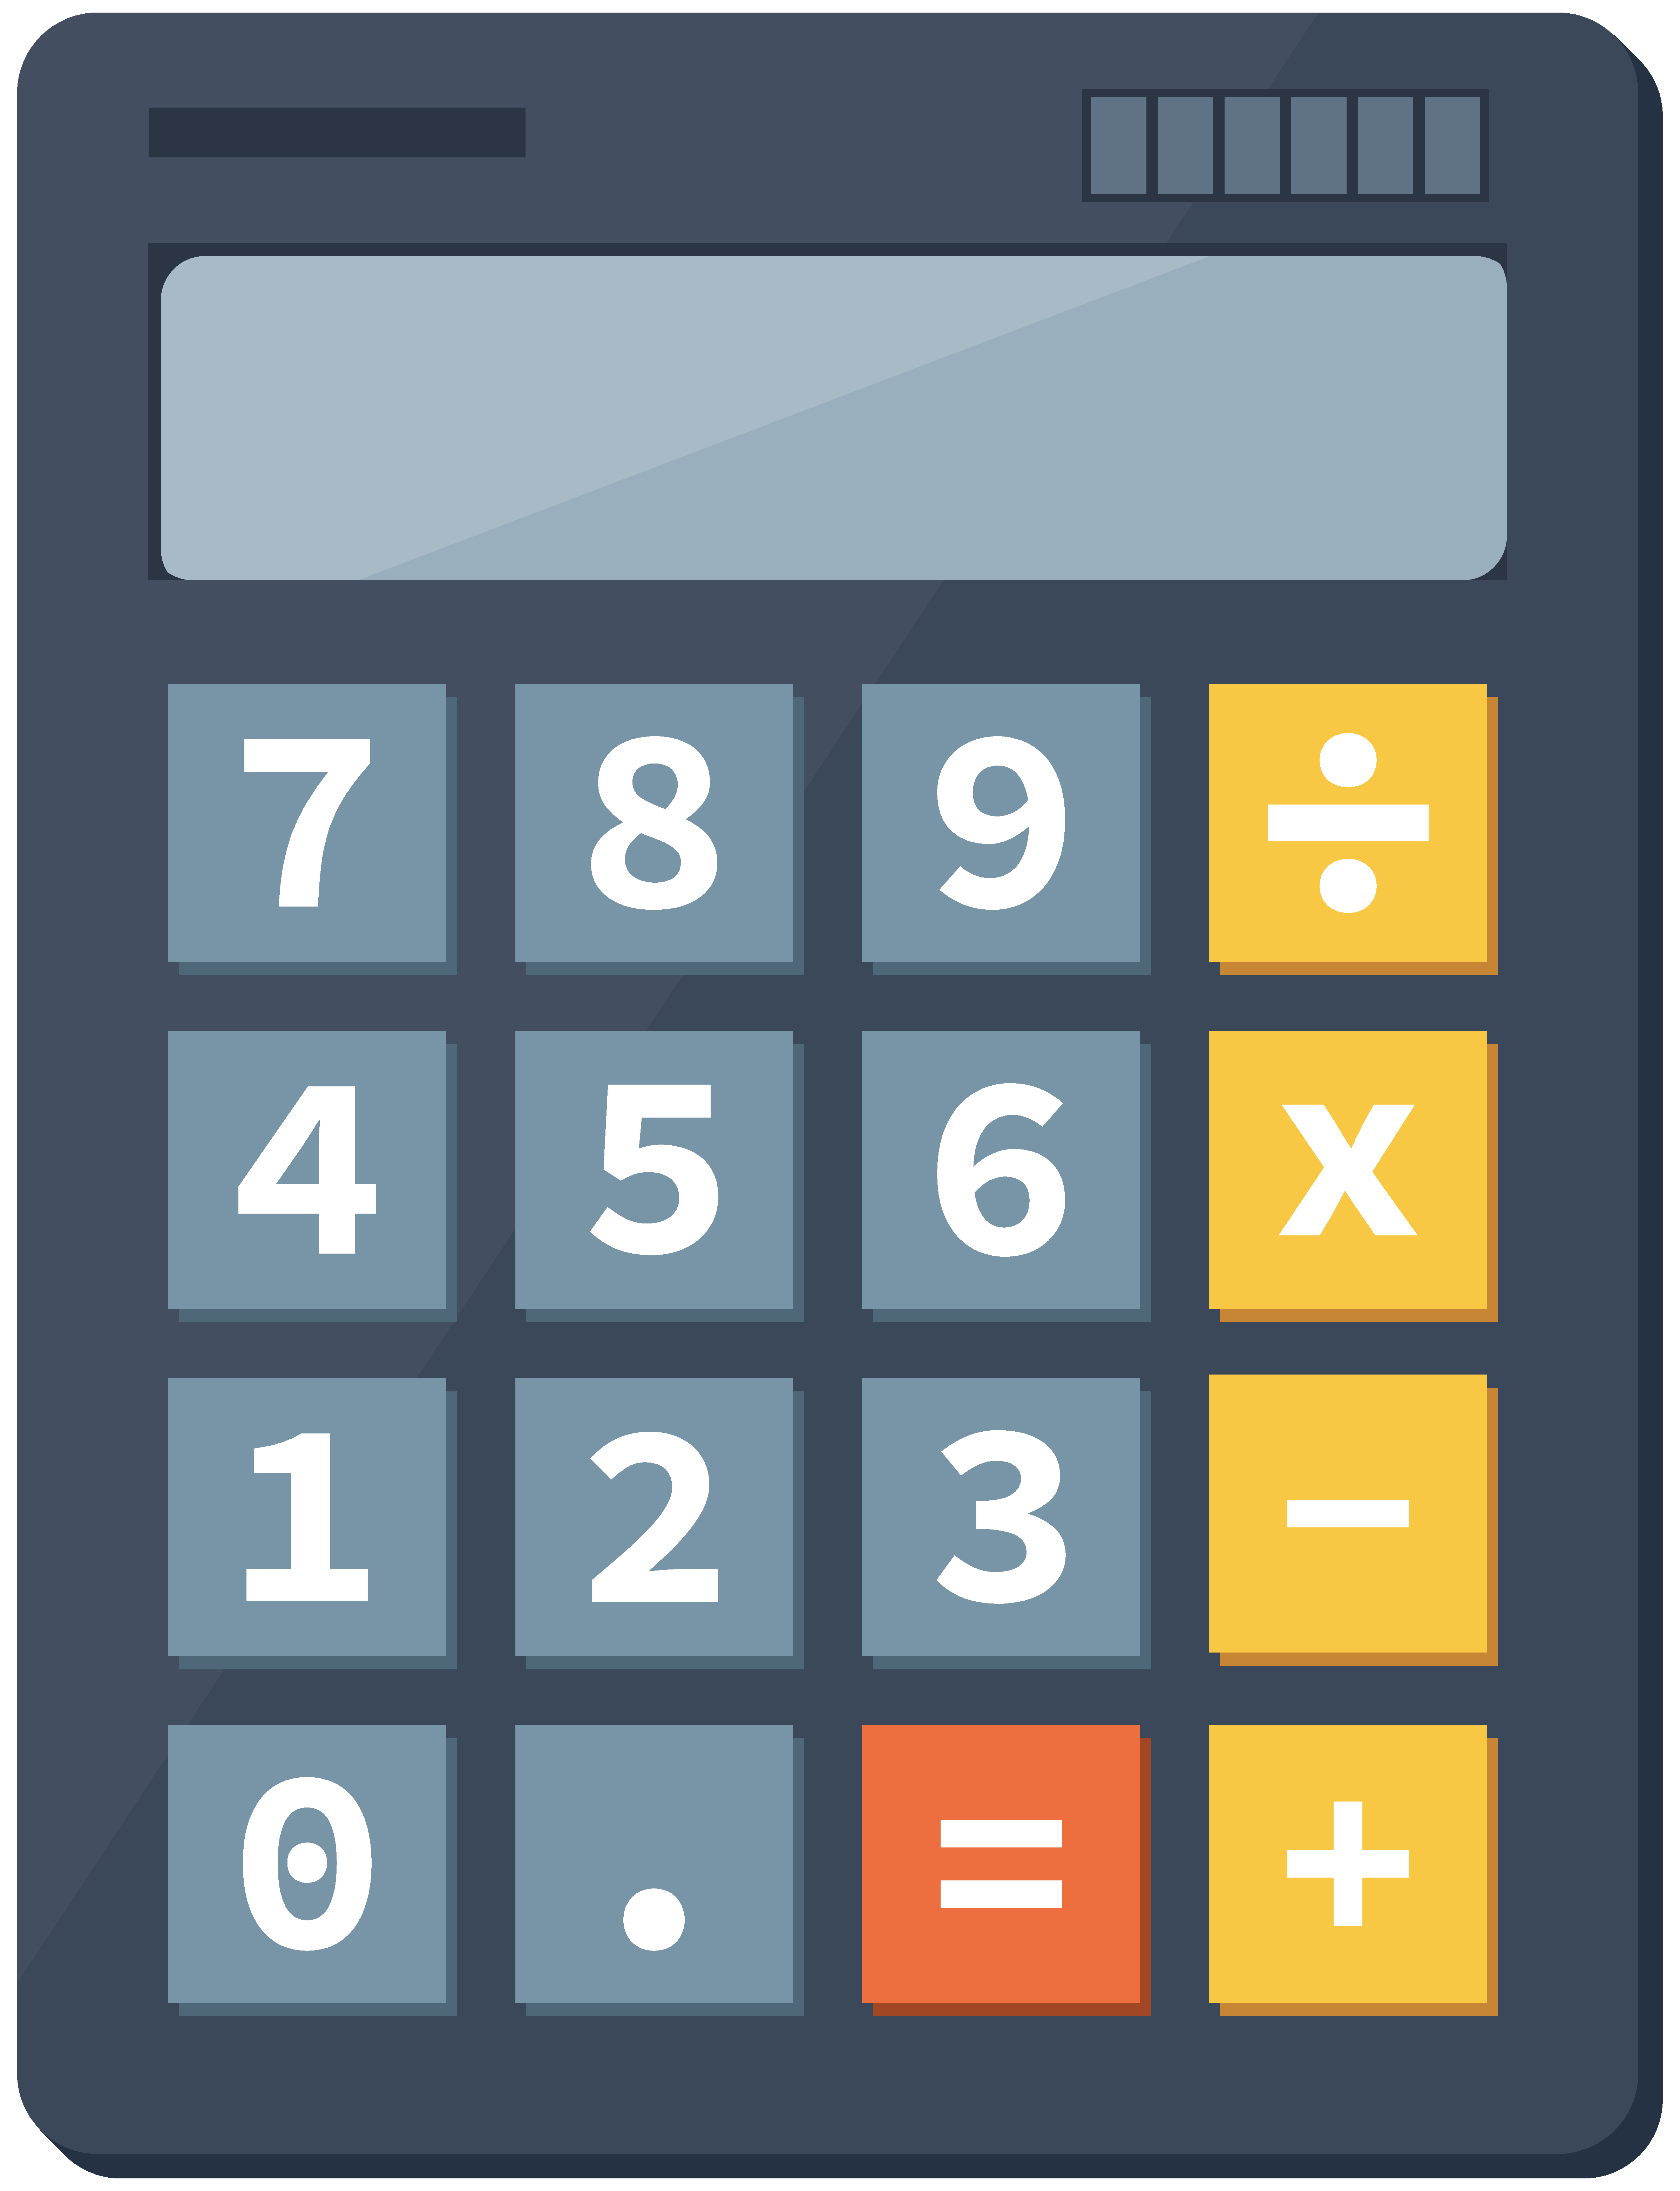
\includegraphics[height=5.7cm]{calculator.pdf}
  \end{center}
  \tableofcontents
  \clearpage
  ~
  \thispagestyle{empty}
  \clearpage

  \input{Natürliche Zahlen}
  \newpage
\section{Addition $a+b$}

% ----------------------------------------------------------------------------
\subsection{Definition}

Die Addition ist eine Rechenoperation der ersten Stufe. Sie basiert auf dem Vorgang des Zusammenfassens von Dingen.

% ----------------------------------------------------------------------------
\subsection{Schreib- und Sprechweise}
Die beiden Zahlen $a$ und $b$, welche addiert werden, heissen \textbf{Summanden}, das Resultat $c$ heisst \textbf{Summe}.

Für die Addition wird das Operationszeichen $+$ verwendet. Wir schreiben
\[
  a + b = c
\]
und sagen «$a$ plus $b$ ist gleich $c$.» oder «Die Summe von $a$ und $b$ ist gleich $c$.»
\begin{example}
  \textbf{Beispiel:} Die Summe von Drei und Fünf ist gleich Acht: $3 + 5 = 8$
\end{example}

% ----------------------------------------------------------------------------
\subsection{Geometrische Interpretation}

Geometrisch gesehen ist eine Addition das aneinanderhängen zweier Längen.
\begin{center}
  \begin{tikzpicture}
    \tkzInit[xmin=0,xmax=9.5]
    \tkzDrawX[label={}]
    \tkzLabelX
    \tkzDefPoint(0,0){O}
    \tkzDefPoint(3,0){A}
    \tkzDefPoint(8,0){C}
    \tkzDrawSegment[dim={$3$,10pt,}](O,A)
    \tkzDrawSegment[dim={$5$,10pt,}](A,C)
    \tkzDrawSegment[dim={$8$,20pt,}](O,C)
  \end{tikzpicture}
\end{center}

So bedeutet $3+5$, dass die Distanz von $0$ zu $3$ und die Distanz von $0$ zu $5$ aneinandergehängt werden. Dabei wird der Punkt $8$ erreicht, also $3+5 = 8$.

% ----------------------------------------------------------------------------
\subsection{Kommutativgesetz}

Anhand der geometrischen Interpretation der Addition ist ersichtlich, dass es keine Rolle spielt, in welcher Reihenfolge die Summanden stehen. Wenn an die Länge $5$ die Länge $3$ angehängt wird, wird der gleiche Ort erreicht wie wenn an die Länge $3$ die Länge $5$ angehängt wird.
\begin{center}
  \begin{tikzpicture}
    \tkzInit[xmin=0,xmax=9.5]
    \tkzDrawX[label={}]
    \tkzLabelX
    \tkzDefPoint(0,0){O}
    \tkzDefPoint(3,0){A}
    \tkzDefPoint(5,0){B}
    \tkzDefPoint(8,0){C}
    \tkzDrawSegment[dim={$3$,10pt,}](O,A)
    \tkzDrawSegment[dim={$5$,10pt,}](A,C)
    \tkzDrawSegment[dim={$5$,20pt,}](O,B)
    \tkzDrawSegment[dim={$3$,20pt,}](B,C)
  \end{tikzpicture}
\end{center}
Diese Erkenntnis wird als mathematisches Gesetz formuliert:
\begin{theorem}
  \textbf{Kommutativgesetz.} Die Summanden einer Addition können vertauscht werden, ohne dass sich der Wert der Summe ändert.
  \[
    a + b = b + a
  \]
\end{theorem}

% ----------------------------------------------------------------------------
\subsection{Assoziativgesetz}

Grundsätzlich werden mehrere Additionen immer \textbf{von links nach rechts} ausgeführt. Um die Reihenfolge zu ändern, können Klammern verwendet werden. Operationen in Klammern werden zuerst ausgeführt.
\begin{example}
  \textbf{Beispiel:} Hier wird von links nach rechts gerechnet:
  \[
    2 + 3 + 4 = 5 + 4 = 9
  \]
  Hier wird zuerst die Addition in den Klammern ausgeführt:
  \[
    2 + (3 + 4) = 2 + 7 = 9
  \]
\end{example}

Offenbar spielt bei Addition diese Reihenfolge keine Rolle. Dies kann wieder anhand der geometrischen Darstellung auf der Zahlengerade gezeigt werden:
\begin{center}
  \begin{tikzpicture}
    \tkzInit[xmin=0,xmax=9.5]
    \tkzDrawX[label={}]
    \tkzLabelX
    \tkzDefPoint(0,0){O}
    \tkzDefPoint(2,0){A}
    \tkzDefPoint(5,0){B}
    \tkzDefPoint(9,0){C}
    \tkzDrawSegment[dim={$2$,12pt,}](O,A)
    \tkzDrawSegment[dim={$3+4$,12pt,}](A,C)
    \tkzDrawSegment[dim={$2+3$,24pt,}](O,B)
    \tkzDrawSegment[dim={$4$,24pt,}](B,C)
  \end{tikzpicture}
\end{center}
Auch diese Erkenntnis wird als mathematisches Gesetz formuliert:
\begin{theorem}
  \textbf{Assoziativgesetz.} Mehrere Additionen dürfen in beliebiger Reihenfolge ausgeführt werden, ohne dass sich der Wert der Summe ändert.
  \[
    a + b + c = (a + b) + c = a + (b + c)
  \]
\end{theorem}

% ----------------------------------------------------------------------------
\subsection{Neutralität der Null}

Die Zahl Null hat bezüglich der Addition eine besondere Stellung. Das Addieren von Null verändert den Wert nicht. Deshalb wird sie \textbf{neutral} bezüglich der Addition genannt.
\begin{theorem}
  \textbf{Neutralität der Null.} Zu einer Zahl kann Null addiert werden, ohne dass sich der Wert ändert:
  \[
    a + 0 = 0 + a = a
  \]
\end{theorem}

  \newpage
\section{Multiplikation $a\cdot b$}

% ----------------------------------------------------------------------------
\subsection{Definition}
Die Multiplikation ist eine Rechenoperation der zweiten Stufe. Das Produkt zweier natürlicher Zahlen $n$ und $a$ entsteht durch das wiederholte Addieren des gleichen Summanden $a$ zum Ausgangswert Null:
\[
  n\cdot a := 0+\underbrace{a+a+\cdots+a}_{n-\text{mal}}
\]
Wenn in dieser Definition $n=0$ gesetzt wird, kommt $a$ gar nicht als Summand vor und das Resultat ist $0$.
\begin{theorem}
  \textbf{Multiplikation mit Null:} Das Produkt einer beliebigen Zahl $a$ und Null ist gleich Null.
  \[
    0 \cdot a = 0
  \]
\end{theorem}

% ----------------------------------------------------------------------------
\subsection{Schreib- und Sprechweise}
Die beiden Zahlen $a$ und $b$, welche multipliziert werden, heissen \textbf{Faktoren}, das Resultat $c$ heisst \textbf{Produkt}.

Für die Multiplikation wird das Zeichen $\cdot$ verwendet. Wir schreiben
\[
  a \cdot b = c
\]
und sagen «$a$ mal $b$ ist gleich $c$.» oder «Das Produkt von $a$ und $b$ ist gleich $c$.»
\begin{example}
  \textbf{Beispiel:} Das Produkt von Zwei und Drei ist gleich Sechs: $2 \cdot 3 = 6$
\end{example}

% ----------------------------------------------------------------------------
\subsection{Geometrische Interpretation}

Geometrisch entspricht das Produkt zweier Zahlen $a\cdot b$ dem Flächeninhalt eines Rechtecks mit den entsprechenden Seiten $a$ und $b$.

Das Produkt dreier Zahlen $a\cdot b\cdot c$ entspricht dem Volumen eines Quaders mit den Seiten $a$, $b$ und $c$.
\begin{center}
  \begin{tikzpicture}[scale=0.8]
    \tkzText(2.5,3.5){$a\cdot b$}
    \tkzDefPoint(0,0){A1}
    \tkzDefPoint(5,0){A2}
    \tkzDefPoint(5,3){A3}
    \tkzDefPoint(0,3){A4}
    \tkzDrawPolygon[fill=lightgreen](A1,A2,A3,A4)
    \tkzLabelLine[below](A1,A2){$a$}
    \tkzLabelLine[left](A1,A4){$b$}
    \foreach \y in {0,...,3}{\tkzDrawSegment({0,\y},{5,\y})}
    \foreach \x in {0,...,5}{\tkzDrawSegment({\x,0},{\x,3})}

    \tkzText(10,3.5){$a\cdot b\cdot c$}
    \tkzDefPoint(7,0){B1}
    \tkzDefPoint(12,0){B2}
    \tkzDefPoint(12,2){B3}
    \tkzDefPoint(7,2){B4}
    \tkzDefPoint(13,1){B5}
    \tkzDefPoint(13,3){B6}
    \tkzDefPoint(8,3){B7}
    \tkzDrawPolygon[fill=lightgreen](B1,B2,B3,B4)
    \tkzDrawPolygon[fill=lightgreen](B2,B5,B6,B3)
    \tkzDrawPolygon[fill=lightgreen](B3,B6,B7,B4)
    \tkzLabelLine[below](B1,B2){$a$}
    \tkzLabelLine[left](B1,B4){$c$}
    \tkzLabelLine[below right](B2,B5){$b$}

    \tkzDrawSegment({12.33,0.33},{12.33,2.33})
    \tkzDrawSegment({12.67,0.67},{12.67,2.67})
    \tkzDrawSegment({7.33,2.33},{12.33,2.33})
    \tkzDrawSegment({7.67,2.67},{12.67,2.67})

    \foreach \y in {0,...,2}{\tkzDrawSegment({7,\y},{12,\y})}
    \foreach \y in {0,...,2}{\tkzDrawSegment({12,\y},{13,\y+1})}
    \foreach \x in {7,...,12}{\tkzDrawSegment({\x,0},{\x,2})}
    \foreach \x in {7,...,12}{\tkzDrawSegment({\x,2},{\x+1,3})}
  \end{tikzpicture}
\end{center}

% ----------------------------------------------------------------------------
\subsection{Kommutativgesetz}

Anhand der geometrischen Interpretation wird ersichtlich, dass auch für die Multiplikation das Kommutativgesetz gelten muss. Das Vertauschen der beiden Faktoren entspricht dem Vertauschen der beiden Seitenlängen eines Rechtecks, was einer Drehung um \ang{90} entspricht. Die Fläche des Rechtecks und somit das Produkt verändert sich dabei nicht.
\begin{center}
  \begin{tikzpicture}[scale=0.8]
    \tkzDefPoint(0,0){A1}
    \tkzDefPoint(4,0){A2}
    \tkzDefPoint(4,3){A3}
    \tkzDefPoint(0,3){A4}
    \tkzDrawPolygon[fill=lightgreen](A1,A2,A3,A4)
    \tkzLabelLine[below](A1,A2){$a$}
    \tkzLabelLine[left](A1,A4){$b$}
    \foreach \y in {0,...,3}{\tkzDrawSegment({0,\y},{4,\y})}
    \foreach \x in {0,...,4}{\tkzDrawSegment({\x,0},{\x,3})}

    \tkzDefPoint(7,-0.5){B1}
    \tkzDefPoint(10,-0.5){B2}
    \tkzDefPoint(10,3.5){B3}
    \tkzDefPoint(7,3.5){B4}
    \tkzDrawPolygon[fill=lightgreen](B1,B2,B3,B4)
    \tkzLabelLine[below](B1,B2){$b$}
    \tkzLabelLine[left](B1,B4){$a$}
    \foreach \y in {0,...,4}{\tkzDrawSegment({7,\y-0.5},{10,\y-0.5})}
    \foreach \x in {0,...,3}{\tkzDrawSegment({\x+7,-0.5},{\x+7,3.5})}
  \end{tikzpicture}
\end{center}
\begin{theorem}
  \textbf{Kommutativgesetz.} Die Faktoren einer Multiplikation dürfen vertauscht werden, ohne dass sich der Wert des Produkts ändert:
  \[
    a \cdot b = b \cdot a
  \]
\end{theorem}

% ----------------------------------------------------------------------------
\subsection{Assoziativgesetz}
Das Volumen eines Quaders ergibt sich aus der Grundfläche multipliziert mit der Höhe. Je nach Orientierung des Quaders ergibt sich somit eine andere Formel für das gleiche Volumen. Wird bei der rechten Formel das Kommutativgesetz angewendet, ergibt sich daraus das Assoziativgesetz für die Multiplikation.
\begin{center}
  \begin{tikzpicture}[scale=0.8]
    \tkzDefPoint(0,0){A1}
    \tkzDefPoint(4,0){A2}
    \tkzDefPoint(4,2){A3}
    \tkzDefPoint(0,2){A4}
    \tkzDefPoint(5,1){A5}
    \tkzDefPoint(5,3){A6}
    \tkzDefPoint(1,3){A7}
    \tkzDrawPolygon[fill=lightgreen](A1,A2,A3,A4)
    \tkzDrawPolygon[fill=lightgreen](A2,A5,A6,A3)
    \tkzDrawPolygon[fill=lightgreen](A3,A6,A7,A4)
    \tkzLabelLine[below](A1,A2){$a$}
    \tkzLabelLine[left](A1,A4){$c$}
    \tkzLabelLine[below right](A2,A5){$b$}

    \tkzDrawSegment({4.33,0.33},{4.33,2.33})
    \tkzDrawSegment({4.67,0.67},{4.67,2.67})
    \tkzDrawSegment({0.33,2.33},{4.33,2.33})
    \tkzDrawSegment({0.67,2.67},{4.67,2.67})

    \foreach \y in {0,...,2}{\tkzDrawSegment({0,\y},{4,\y})}
    \foreach \y in {0,...,2}{\tkzDrawSegment({4,\y},{5,\y+1})}
    \foreach \x in {0,...,4}{\tkzDrawSegment({\x,0},{\x,2})}
    \foreach \x in {0,...,4}{\tkzDrawSegment({\x,2},{\x+1,3})}

    \tkzDefPoint(7,0){B1}
    \tkzDefPoint(10,0){B2}
    \tkzDefPoint(10,4){B3}
    \tkzDefPoint(7,4){B4}
    \tkzDefPoint(10.67,0.67){B5}
    \tkzDefPoint(10.67,4.67){B6}
    \tkzDefPoint(7.67,4.67){B7}
    \tkzDrawPolygon[fill=lightgreen](B1,B2,B3,B4)
    \tkzDrawPolygon[fill=lightgreen](B2,B5,B6,B3)
    \tkzDrawPolygon[fill=lightgreen](B3,B6,B7,B4)
    \tkzLabelLine[below](B1,B2){$b$}
    \tkzLabelLine[left](B1,B4){$a$}
    \tkzLabelLine[below right](B2,B5){$c$}

    \tkzDrawSegment({10.33,0.33},{10.33,4.33})
    \tkzDrawSegment({10.67,0.67},{10.67,4.67})
    \tkzDrawSegment({7.33,4.33},{10.33,4.33})
    \tkzDrawSegment({7.67,4.67},{10.67,4.67})

    \foreach \y in {0,...,4}{\tkzDrawSegment({7,\y},{10,\y})}
    \foreach \y in {0,...,4}{\tkzDrawSegment({10,\y},{10.67,\y+0.67})}
    \foreach \x in {7,...,10}{\tkzDrawSegment({\x,0},{\x,4})}
    \foreach \x in {7,...,10}{\tkzDrawSegment({\x,4},{\x+0.67,4.67})}

    \tkzText(3,3.5){$a\cdot b\cdot c$}
    \tkzText[black](9,5.2){$b\cdot c\cdot a = a\cdot (b\cdot c)$}
  \end{tikzpicture}
\end{center}
\begin{theorem}
  \textbf{Assoziativgesetz.} Mehrere Multiplikationen dürfen in beliebiger Reihenfolge ausgeführt werden, ohne dass sich der Wert des Produkts ändert:
  \[
    a \cdot b \cdot c = (a \cdot b) \cdot c = a \cdot (b \cdot c)
  \]
\end{theorem}

% ----------------------------------------------------------------------------
\subsection{Neutralität der Eins}

Die Eins hat bezüglich der Multiplikation eine besondere Stellung. Das Multiplizieren mit Eins verändert den Wert nicht.
\begin{theorem}
  \textbf{Neutralität der Eins.} Eine Zahl kann mit Eins multipliziert werden, ohne dass sich der Wert ändert:
  \[
    a \cdot 1 = 1 \cdot a = a
  \]
\end{theorem}


% ----------------------------------------------------------------------------
\subsection{Distributivgesetz}
Das Distributivgesetz verbindet die Addition und die Multiplikation. Es kann ebenfalls durch eine geometrische Überlegung begründet werden. Wird das Rechteck mit den Seiten $a$ und $b$ und das Rechteck mit den Seiten $a$ und $c$ zusammengesetzt, so ergibt sich ein Rechteck mit den Seiten $a$ und $b+c$, welches die gleiche Fläche wie die beiden ersten Rechtecke hat.
\begin{center}
  \begin{tikzpicture}[scale=0.8]
    \tkzText(3,3.5){$a\cdot b+a\cdot c$}
    \tkzDefPoint(0,0){A1}
    \tkzDefPoint(3,0){A2}
    \tkzDefPoint(3,3){A3}
    \tkzDefPoint(0,3){A4}
    \tkzDrawPolygon[fill=lightgreen](A1,A2,A3,A4)
    \tkzLabelLine[below](A1,A2){$b$}
    \tkzLabelLine[left](A1,A4){$a$}
    \foreach \y in {0,...,3}{\tkzDrawSegment({0,\y},{3,\y})}
    \foreach \x in {0,...,3}{\tkzDrawSegment({\x,0},{\x,3})}

    \tkzDefPoint(4,0){B1}
    \tkzDefPoint(6,0){B2}
    \tkzDefPoint(6,3){B3}
    \tkzDefPoint(4,3){B4}
    \tkzDrawPolygon[fill=lightgreen](B1,B2,B3,B4)
    \tkzLabelLine[below](B1,B2){$c$}
    \tkzLabelLine[left](B1,B4){$a$}
    \foreach \y in {0,...,3}{\tkzDrawSegment({4,\y},{6,\y})}
    \foreach \x in {4,...,6}{\tkzDrawSegment({\x,0},{\x,3})}

    \tkzText(10.5,3.5){$a\cdot(b+c)$}
    \tkzDefPoint(8,0){C1}
    \tkzDefPoint(13,0){C2}
    \tkzDefPoint(13,3){C3}
    \tkzDefPoint(8,3){C4}
    \tkzDrawPolygon[fill=lightgreen](C1,C2,C3,C4)
    \tkzLabelLine[below](C1,C2){$b+c$}
    \tkzLabelLine[left](C1,C4){$a$}
    \foreach \y in {0,...,3}{\tkzDrawSegment({8,\y},{13,\y})}
    \foreach \x in {8,...,13}{\tkzDrawSegment({\x,0},{\x,3})}
  \end{tikzpicture}
\end{center}

\begin{theorem}
  \textbf{Distributivgesetz.} Eine Summe wird mit einem Faktor $a$ multipliziert, indem jeder Summand mit $a$ multipliziert wird.
  \[
    a \cdot (b + c) = a \cdot b + a \cdot c
  \]
\end{theorem}

  \newpage
\section{Potenzieren $a^{b}$}

% ----------------------------------------------------------------------------
\subsection{Definition}

Das Potenzieren ist eine Rechenoperation der dritten Stufe. Die Potenz zweier natürlicher Zahlen entsteht durch das wiederholte Multiplizieren des gleichen Faktors $a$ mit dem Ausgangswert Eins:
\[
  a^{n} := 1\cdot\underbrace{a\cdot a\cdot a\cdots a}_{n-\text{mal}}
\]

Wenn in dieser Definition $n=0$ gesetzt wird, kommt $a$ gar nicht als Faktor vor und das Resultat ist $1$.
\begin{theorem}
  \textbf{Potenzieren mit Null:} Die nullte Potenz einer von Null verschiedenen Zahl $a$ ist gleich Eins.
  \[
    a^{0} = 1 \qquad a \ne 0
  \]
\end{theorem}

% ----------------------------------------------------------------------------
\subsection{Schreib- und Sprechweise}
Die Zahl $a$, welche potenziert wird, heisst \textbf{Basis}. Die Zahl $b$, um welche potenziert wird, heisst \textbf{Exponent}. Das Resultat einer Potenzierung heisst \textbf{Potenz}.

Für das Potenzieren wird kein Operationszeichen verwendet. Stattdessen wird der Exponent $b$ hochgestellt nach der Basis $a$ geschrieben:
\[
  a^{b} = c
\]
und sagen «$a$ hoch $b$ ist gleich $c$.» oder «Die $b$-te Potenz von $a$ ist gleich $c$.

\begin{example}
  \textbf{Beispiel:} Die vierte Potenz von Drei ist gleich $81$:
  \[
    3^{4} = 81
  \]
\end{example}

Das Potenzieren mit Zwei wird als \textbf{Quadrieren} bezeichnet, das Resultat dieser Operation als \textbf{Quadrat}.

\begin{example}
  \textbf{Beispiel:} Das Quadrat von Fünf ist gleich $25$:
  \[
    5^{2} = 25
  \]
\end{example}

\begin{note}
  \textbf{Achtung:} Für das Potenzieren gibt es weder ein Kommutativ- noch ein Assoziativgesetz.
  \[
    8 = 2^{3} \ne 3^{2} = 9 \qquad\qquad 8 = 2^{3} = \left(2^{1}\right)^{3} \ne 2^{(1^{3})} = 2^{1} = 2
  \]
\end{note}

\newpage
% ----------------------------------------------------------------------------
\subsection{Reihenfolge der Operationen}

Damit bei einer Rechenanweisung wie $2+3\cdot 5^{2}$ immer das gleiche Resultat entsteht, muss die Reihenfolge, in welcher die Operationen ausgeführt werden, klar geregelt werden. Dabei gelten folgende Vorschriften:

\textbf{Klammern zuerst.} Zuerst werden immer Operationen innerhalb von Klammern ausgeführt. Bei mehreren verschachtelten Klammern wird immer zuerst die innerste Klammer ausgerechnet.

\begin{example}
  \textbf{Beispiele:}
  \[
    5\cdot (2+3) = 5\cdot 5 = 25 \qquad\qquad (2\cdot 3)^{2} = 6^{2} = 36
  \]
\end{example}

\textbf{Dritte Stufe.} Danach werden Operationen der dritten Stufe ausgeführt, also Potenzieren und Wurzelziehen. Verschachtelte Potenzen werden von \textbf{oben nach unten} ausgeführt.

\begin{example}
  \textbf{Beispiele:}
  \[
    2\cdot 3^{2} = 2\cdot 9 = 18 \qquad\qquad 2^{3^{2}} = 2^{9} = 512 \qquad\qquad \left(2^{3}\right)^{2} = 8^{2} = 64
  \]
\end{example}

\begin{note}
  \textbf{Achtung:} Einfache Taschenrechner beachten diese Regel nicht und führen verschachtelte Potenzen von links nach rechts aus.
\end{note}

\textbf{Zweite Stufe (Punktoperationen).} Danach werden Operationen der zweiten Stufe ausgeführt, also Multiplikationen und Divisionen. Mehrere aufeinanderfolgende Operationen auf dieser Stufe werden von \textbf{links nach rechts} ausgeführt.

\begin{example}
  \textbf{Beispiele:}
  \[
    5\cdot 2+3 = 10+3 = 13 \qquad\qquad 2\cdot 3\cdot 4 = 6\cdot 4 = 24
  \]
\end{example}

\textbf{Erste Stufe (Strichoperationen).} Danach werden Operationen der ersten Stufe ausgeführt, also Additionen und Subtraktionen. Mehrere aufeinanderfolgende Operationen auf dieser Stufe werden von \textbf{links nach rechts} ausgeführt.

\begin{example}
  \textbf{Beispiele:}
  \[
    2+3+4 = 5+4 = 9 \qquad\qquad 2+(3+4) = 2+7 = 9
  \]
\end{example}

  \newpage
\section{Teiler und Primzahlen}

% ----------------------------------------------------------------------------
\subsection{Teiler}

\textbf{Definition:} Die natürliche Zahl $t$ ist ein \textbf{Teiler} der natürlichen Zahl $n$, wenn $n$ ohne Rest durch $t$ dividiert werden kann, also wenn es genau eine natürliche Zahl $z$ gibt, sodass gilt:
  \[
    t\cdot z = n
  \]
Wir schreiben $t\mid n$ und sagen «$t$ ist ein Teiler von $n$» oder «$t$ teilt $n$».

\begin{example}
  \textbf{Beispiele:}
  \begin{itemize}[noitemsep]
    \item Die Zahl $60$ hat $12$ Teiler, nämlich $1, 2, 3, 4, 5, 6, 10, 12, 15, 20, 30$ und $60$.
    \item Die Zahl $13$ hat zwei Teiler, nämlich $1$ und $13$.
    \item Die Zahl $1$ teilt jede natürliche Zahl.
    \item Die Zahl $0$ teilt keine natürliche Zahl.
    \item Die Zahl $0$ hat jede natürliche Zahl ausser sich selbst als Teiler.
  \end{itemize}
\end{example}

Zwei Zahlen heissen \textbf{teilerfremd}, wenn sie ausser $1$ keinen gemeinsamen Teiler haben.

% ----------------------------------------------------------------------------
\subsection{Primzahlen}

\textbf{Definition.} Eine natürliche Zahl ist \textbf{prim} oder eine \textbf{Primzahl}, wenn sie genau zwei Teiler hat.

Die beiden Teiler sind Eins und die Zahl selbst. Somit ist die Zahl Eins keine Primzahl, da sie nur einen Teiler hat.

Die Zwei ist die kleinste Primzahl und gleichzeitig die einzige gerade Primzahl. Alle anderen geraden Zahlen haben ja neben Eins und sich selbst noch mindestens die Zwei als Teiler und haben somit mehr als zwei Teiler.

% ----------------------------------------------------------------------------
\subsection{Sieb des Eratosthenes}

Das Sieb des Eratosthenes ist ein Algorithmus, um alle Primzahlen in einem bestimmten Zahlenbereich zu finden.

Dazu werden alle Zahlen von $2$ bis zur gewünschten maximalen Zahl aufgeschrieben. Dann werden folgende Anweisungen immer wiederholt, bis alle Zahlen eingefärbt oder Primzahlen sind:
\begin{enumerate}
  \item Nimm die kleinste nicht eingefärbte Zahl. Das ist eine Primzahl.
  \item Färbe alle Vielfachen dieser Zahl ein.
  \item Beginne von vorne.
\end{enumerate}

\newpage
% ----------------------------------------------------------------------------
\subsection{Primfaktorzerlegung}

\begin{theorem}
  \textbf{Satz:} Zu jeder natürlichen Zahl $n$ existiert eine eindeutige Primfaktorzerlegung
  \[
    n = p_{1}^{r_{1}} \cdot p_{2}^{r_{2}} \cdot \cdots \cdot p_{s}^{r_{s}}
  \]
  Dabei sind $p_{1}, p_{2}, \ldots, p_{s}$ die ersten $s$ Primzahlen. Die Potenzen $r_{1}, r_{2},\ldots, r_{s}$ geben an, wie oft die jeweilige Primzahl als Faktor in n vorkommt.
\end{theorem}

\begin{example}
  \textbf{Beispiel:}
  \[
    504 = 2\cdot 2\cdot 2\cdot 3\cdot 3\cdot 7 = 2^{3}\cdot 3^{2}\cdot 7
  \]
\end{example}

Eine wichtige Anwendung der Primfaktorzerlegung ist das Kürzen und Erweitern von Brüchen. Angenommen, der folgende Bruch soll gekürzt werden:
\[
  \frac{14014}{5278}
\]
Zunächst werden Zähler und Nenner in ihre Primfaktoren zerlegt. Gemeinsame Primfaktoren in Zähler und Nenner können gekürzt werden:
\[
  \frac{14014}{5278} = \frac{2\cdot 7\cdot 7\cdot 11\cdot 13}{2\cdot 7\cdot 13\cdot 29} = \frac{7\cdot 11}{29} = \frac{77}{29}
\]

% ----------------------------------------------------------------------------
\subsection{Aufwand der Primfaktorzerlegung}

Das Zerlegen einer grossen Zahl in ihre Primfaktoren ist sehr aufwändig, weil es bis heute keinen effizienten Algorithmus dafür gibt. Je nach Grösse der Zahl dauert eine solche vom Computer durchgeführte Zerlegung Stunden, Tage, Jahre oder gar Milliarden von Jahren. Beispielsweise wurde die Zahl RSA-240, eine 240-stellige Zahl, im November 2019 von einem Zusammenschluss von Computern zerlegt; auf einem Single-core-Rechner hätte die Faktorisierung etwa 900 Jahre in Anspruch genommen.

In der Informatik basieren wichtige Verschlüsselungsverfahren darauf, dass es unmöglich ist, eine grosse Zahl in vernünftiger Zeit in ihre Primfaktoren zu zerlegen.

% ----------------------------------------------------------------------------
\subsection{ggT und kgV}

Den grössten gemeinsamen Teiler (ggT) und das kleinste gemeinsame Vielfache (kgV) zweier Zahlen kann mit Hilfe der Primfaktorzerlegung der beiden Zahlen ermittelt werden.
\begin{align*}
  6468 &= 2\cdot2\cdot3\cdot7\cdot7\cdot11 = 2^{2}\cdot 3\cdot 7^{2}\cdot 11 \\
   840 &= 2\cdot2\cdot2\cdot3\cdot5\cdot7 = 2^{3}\cdot 3\cdot 5\cdot 7
\end{align*}
Der grösste gemeinsame Teiler ist das Produkt aller Primfaktoren, welche in beiden Zerlegungen vorkommen.
\begin{center}
  \renewcommand{\arraystretch}{1.3}
  \begin{tabular}{rccccccccccccccc}
    \hline
      $6488=$ & \cellcolor{lightgreen} $2$ & $\cdot$ & \cellcolor{lightgreen} $2$ & $\cdot$ & & & \cellcolor{lightgreen} $3$ & $\cdot$ & & & \cellcolor{lightgreen} $7$ & $\cdot$ & $7$ & $\cdot$ & $11$ \\
    \hline
       $840=$ & \cellcolor{lightgreen} $2$ & $\cdot$ & \cellcolor{lightgreen} $2$ & $\cdot$ & $2$ & $\cdot$ & \cellcolor{lightgreen} $3$ & $\cdot$ & $5$ & $\cdot$ & \cellcolor{lightgreen} $7$ & & & & \\
    \hline
  \end{tabular}
\end{center}
Also ist $\ggT(6488;840) = 2\cdot2\cdot 3\cdot 7 = 84$.

Für das kleinste gemeinsame Vielfache müssen diejenigen Primfaktoren gesucht werden, die in mindestens einer der beiden Zerlegungen vorkommen:
\begin{center}
  \renewcommand{\arraystretch}{1.3}
  \begin{tabular}{rccccccccccccccc}
    \hline
      $6488=$ & \cellcolor{lightgreen} $2$ & $\cdot$ & \cellcolor{lightgreen} $2$ & $\cdot$ & & & \cellcolor{lightgreen} $3$ & $\cdot$ & & & \cellcolor{lightgreen} $7$ & $\cdot$ & \cellcolor{lightgreen} $7$ & $\cdot$ & \cellcolor{lightgreen} $11$ \\
    \hline
       $840=$ & $2$ & $\cdot$ & $2$ & $\cdot$ & \cellcolor{lightgreen} $2$ & $\cdot$ & $3$ & $\cdot$ & \cellcolor{lightgreen} $5$ & $\cdot$ & $7$ & & & & \\
    \hline
  \end{tabular}
\end{center}
Also ist $\kgV(6468;840) = 2\cdot2\cdot2\cdot5\cdot7\cdot7\cdot11 = 64680$.

% ----------------------------------------------------------------------------
\subsection{Wie viele Primzahlen gibt es?}

Bereits der griechische Mathematiker Euklid von Alexandria (ca. 300 v.Chr.) hat bewiesen, dass es unendlich viele Primzahlen gibt. Da damals das Konzept der Unendlichkeit noch nicht bekannt war, hat er seinen Satz und den Beweis so formuliert:

\begin{quote}
  «Es gibt mehr Primzahlen als jede vorgelegte Anzahl Primzahlen.»
\end{quote}

Wird sein Satz in moderne Sprache übersetzt, lautet er so:
\begin{theorem}
  \textbf{Satz des Euklid:} Es gibt unendlich viele Primzahlen.
\end{theorem}

Um diesen Satz zu beweisen, muss gezeigt werden, dass zur jeder Primzahl $p$ eine grössere Primzahl gefunden werden kann. Euklid hat den Satz wie folgt bewiesen:

Es wird angenommen, dass alle Primzahlen bis zur Primzahl $p$ bekannt sind:
\[
  2, 3, 5, 7, 11, 13, \ldots, p
\]
Nun werden alle diese Primzahlen miteinander multipliziert und zu Eins addiert:
\[
  z = 1 + 2\cdot 3\cdot 5\cdot 7\cdot 11\cdot 13\cdot\cdots\cdot p
\]
Nun werden die Primfaktoren der so entstandenen Zahl $z$ gesucht, indem versucht wird, $z$ durch die bekannten Primzahlen zu dividieren. Bei der Division durch 2 bleibt der Rest übrig, da Eins addiert wurde:
\[
  z:2 = (1 + 2\cdot 3\cdot 5\cdot 7\cdot 11\cdot 13\cdot\cdots\cdot p):2 = \frac{1}{2}+ 3\cdot 5\cdot 7\cdot 11\cdot 13\cdot\cdots\cdot p
\]
Das gleiche lässt sich für alle anderen Primzahlen von 3 bis $p$ feststellen.

Die Primfaktoren von $z$ müssen also Primzahlen sein, die grösser als $p$ sind. Damit ist bewiesen worden, dass zu jeder Primzahl $p$ eine grössere Primzahl gefunden werden kann.

  \newpage
\section{Stellenwertsystem}

% ----------------------------------------------------------------------------
\subsection{Römische Zahlen}

Die Römer haben als Zeichen für die Zahlen die lateinischen Buchstaben verwendet. Dabei hat jeder Buchstaben einen bestimmten Wert:

\begin{center}
  \newcolumntype{C}{>{\centering\arraybackslash}X}
  \begin{tabularx}{0.9\textwidth}{CCCCCCC}
  \toprule
   $\text{I}$ & $\text{V}$ & $\text{X}$ & $\text{L}$ & $\text{C}$ &  $\text{D}$ & $\text{M}$ \\
  \midrule
    $1$        & $5$        & $10$       & $50$       & $100$      & $500$      & $1000$ \\
  \bottomrule
  \end{tabularx}
\end{center}

In einer römischen Zahl werden die Ziffern immer nach absteigendem Wert angeordnet. Ganz links befindet sich die grösste Ziffer, ganz rechts die kleinste.

Um den Wert einer römischen Zahl herauszufinden, müssen nur die Werte der einzelnen Ziffern addiert werden:
\[
  \text{MDCCCCLXXXIIII} = 1000 + 500 + 4\cdot 100 + 50 + 3\cdot 10 + 4 \cdot 1 = 1984
\]
Zusätzlich kann die Subtraktionsregel angewendet werden: Wenn eine kleinere Ziffer links von einer fünf- oder zehnmal grösseren Ziffer steht, so wird die kleiner von der grösseren subtrahiert. Die Zahlen $40$ und $90$ können also so geschrieben werden:
\[
  40 = \text{XXXX} = \text{XL} \qquad\qquad 90 = \text{LXXXX} = \text{XC}
\]
Damit lassen sich die Zahlen kürzer darstellen. Die Zahl $1984$ kann man also so schreiben:
\[
  \text{MCMLXXXIV} = 1000 + (-1\cdot 100 + 1000) + 50 + 3\cdot 10 + (-1 + 5) = 1984
\]

% ----------------------------------------------------------------------------
\subsection{Dezimalsystem}

Wir können sämtliche Zahlen mit den zehn Ziffern $0, 1, 2, 3, 4, 5, 6, 7, 8, 9, 0$ darstellen. Damit so beliebige Werte dargestellt werden können, erhält jede \textbf{Ziffer} je nach ihrer Position oder \textbf{Stelle} in der Zahl einen anderen Wert, ihren \textbf{Stellenwert}, welcher sich aus Zehn hoch die Nummer der Stelle ergibt. Die Stellen werden von rechts nach links durchnummeriert, beginnend bei Null.

Der Wert der Zahl ergibt sich, indem jede Ziffer mit ihrem Stellenwert multipliziert wird und anschliessend alle diese Werte addiert werden. Die Zahl $5478$ bedeutet also, dass $5$ Tausender, $4$ Hunderter, $7$ Zehner und $8$ Einer addiert werden:
\begin{center}
  \renewcommand{\arraystretch}{1}
  \newcolumntype{C}{>{\centering\arraybackslash}X}
  \begin{tabularx}{0.9\textwidth}{lCCCC}
  \toprule
    Stelle & $3$ & $2$ & $1$ & $0$ \\
  \midrule
    Stellenwert (Potenz) & $10^{3}$ & $10^{2}$ & $10^{1}$ & $10^{0}$ \\
  \midrule
    Stellenwert & $1000$ & $100$ & $10$ & $1$ \\
  \midrule
    Ziffer & $5$ & $4$ & $7$ & $8$ \\
  \midrule
    Wert & $5\cdot 1000$ & $4\cdot 100$ & $7\cdot 10$ & $8\cdot 1$ \\
  \bottomrule
  \end{tabularx}
\end{center}

% ----------------------------------------------------------------------------
\subsection{Zahlensysteme mit anderer Basis}

Wir können anstelle der Zahl Zehn eine andere Zahl als \textbf{Basis} der Potenzen und somit des Zahlensystems wählen. Damit verändern sich die Stellenwerte entsprechend.

Dabei stimmt die \textbf{Basis des Zahlensystems} immer mit der Anzahl Ziffern überein.

Damit wir einer Zahl ansehen, in welchem Zahlensystem sie geschrieben wurde, hängen wir die Basis immer tiefgestellt und in Klammern an die Zahl an. Die Zahl «4032» im Fünfersystem schreiben wir:
\[
  4032_{(5)}
\]
Die folgende Abbildung zeigt, wie der Wert der Zahl $4032_{(5)}$ berechnet wird:
\begin{center}
  \newcolumntype{C}{>{\centering\arraybackslash}X}
  \begin{tabularx}{0.9\textwidth}{lCCCC}
  \toprule
    Stelle & $3$ & $2$ & $1$ & $0$ \\
  \midrule
    Stellenwert (Potenz) & $5^{3}$ & $5^{2}$ & $5^{1}$ & $5^{0}$ \\
  \midrule
    Stellenwert & $125$ & $25$ & $5$ & $1$ \\
  \midrule
    Ziffer & $4$ & $0$ & $3$ & $2$ \\
  \midrule
    Wert & $4\cdot 125$ & $0\cdot 25$ & $3\cdot 5$ & $2\cdot 1$ \\
  \bottomrule
  \end{tabularx}
\end{center}

Die Zahl $4032_5$ im Fünfersystem entspricht also der Zahl $517$ im Dezimalsystem:
\[
  4\cdot 125+0\cdot 25+3\cdot 5+2\cdot 1 = 500+9+2 = 517
\]

% ----------------------------------------------------------------------------
\subsection{Übersicht Zahlensysteme}

Hier ist eine Übersicht der Zahlensysteme mit einer Basis von Zwei bis Zehn:
\begin{center}
  \renewcommand{\arraystretch}{1.3}
  \begin{tabularx}{0.7\textwidth}{Xcl}
    \toprule
      \textbf{Bezeichnung}   & \textbf{Basis} & \textbf{Ziffern} \\
    \midrule
      \textbf{Binärsystem}   & $2$     & $0, 1$                      \\
      Dreiersystem           & $3$     & $0, 1, 2$                      \\
      Vierersystem           & $4$     & $0, 1, 2, 3$                   \\
      Fünfersystem           & $5$     & $0, 1, 2, 3, 4$                \\
      Sechsersystem          & $6$     & $0, 1, 2, 3, 4, 5$             \\
      Siebnersystem          & $7$     & $0, 1, 2, 3, 4, 5, 6$          \\
      \textbf{Oktalsystem}   & $8$     & $0, 1, 2, 3, 4, 5, 6, 7$       \\
      Neunersystem           & $9$     & $0, 1, 2, 3, 4, 5, 6, 7, 8$    \\
      \textbf{Dezimalsystem} & $10$    & $0, 1, 2, 3, 4, 5, 6, 7, 8, 9$ \\
    \bottomrule
  \end{tabularx}
\end{center}

  \newpage
\section{Subtraktion $a-b$}

% ----------------------------------------------------------------------------
\subsection{Definition}

Welche Zahl muss zu Fünf addiert werden, um Sieben zu erhalten?
\[
  5 + \square = 7
\]
Um diese Frage zu beantworten, muss die \textbf{Differenz} zwischen Fünf und Sieben bestimmt werden. Die Differenz zweier Zahlen wird mit Hilfe einer \textbf{Subtraktion} berechnet:
\[
  7 - 5 = \square
\]
\textbf{Definition:} Die Subtraktion ist die Umkehroperation der Addition. Mit der Subtraktion wird der unbekannte Summand $x$ einer Addition berechnet:

\begin{align*}
  a+x &= c \\
    x &= c-a
\end{align*}

% ----------------------------------------------------------------------------
\subsection{Schreib- und Sprechweise}

Die Zahl $a$, von welcher subtrahiert wird, heisst \textbf{Minuend}. Die Zahl $b$, welche subtrahiert wird, heisst \textbf{Subtrahend}. Das Resultat einer Subtraktion wird \textbf{Differenz} genannt.

Für die Subtraktion wird das Operationszeichen $-$ verwendet. Wir schreiben
\[
  a - b = c
\]
und sagen «die Differenz von $a$ und $b$ ist gleich $c$.»

% ----------------------------------------------------------------------------
\subsection{Reihenfolge der Operationen}

Die Subtraktion ist eine Operation der ersten Stufe. Das bedeutet, dass Subtraktionen immer gleichzeitig mit den Additionen von links nach rechts ausgeführt werden.

\begin{example}
  \textbf{Beispiele:}
  \begin{align*}
      3-2+1 &= 1+1 = 2 &   5-2\cdot 2 &= 5-4 = 1 \\
    3-(2+1) &= 3-3 = 0 & (5-2)\cdot 2 &= 3\cdot 2 = 6
  \end{align*}
\end{example}

\begin{note}
  \textbf{Achtung:} Für die Subtraktion gibt es weder ein Kommutativ- noch ein Assoziativgesetz.
  \[
    -1 = 2-3 \ne 3-2 = 1 \qquad\qquad 0 = 1-1 = 3-2-1 \ne 3-(2-1) = 3-1 = 2
  \]
\end{note}

  \newpage
\section{Ganze Zahlen $\mathbb{Z}$}

% ----------------------------------------------------------------------------
\subsection{Definition}

Welche Zahl muss zu Fünf addiert werden, um Null zu erhalten?
\[
  5 + \square = 0
\]
Wenn nur die natürlichen Zahlen betrachtet werden, gibt es keine Antwort auf diese Frage. Wenn in der Mathematik eine Lücke entdeckt wird, dann wird oft etwas neues definiert, das heisst «erfunden», um diese Lücke zu füllen.

In diesem Fall werden neue Zahlen definiert, welche diese Gleichung erfüllen.

\textbf{Definition:} Eine Zahl, welche Null ergibt, wenn sie zu einer gegebenen Zahl $a$ addiert wird, wird \textbf{Gegenzahl} von $a$ genannt und mit $-a$ bezeichnet:
\[
  a + (-a) = 0
\]
Die Gegenzahl von $5$ ist also $-5$ und $5 + (-5) = 0$. Wird die Menge der natürlichen Zahlen um ihre Gegenzahlen erweitert, so ergibt sich die Menge der \textbf{ganzen Zahlen}.

\textbf{Definition:} Die Menge der ganzen Zahlen $\mathbb{Z}$ enthält sämtliche natürliche Zahlen sowie ihre Gegenzahlen.
\[
  \mathbb{Z} = \{\ldots -4, -3, -2, -1, 0, 1, 2, 3, 4, \ldots\}
\]

% ----------------------------------------------------------------------------
\subsection{Zahlengerade und Betrag}

Auch die ganzen Zahlen können auf der Zahlengeraden dargestellt werden. Dabei wird die Gegenzahl jeder Zahl gegenüberliegend der Null dargestellt. So wird die Zahl $-4$ auf der anderen Seite von Null mit gleichem Abstand zur Null wie die Zahl $4$ dargestellt.
\begin{center}
  \begin{tikzpicture}
    \tkzInit[xmin=-5.5,xmax=5.5]
    \tkzDrawX[label={}]
    \tkzLabelX
    \tkzDefPoint(0,0){O}
    \tkzDefPoint(-4,0){A}
    \tkzDefPoint(4,0){B}
    \tkzDrawSegment[dim={$4$,10pt,}](A,O)
    \tkzDrawSegment[dim={$4$,10pt,}](O,B)
  \end{tikzpicture}
\end{center}

Der Abstand einer Zahl $a$ zur Null auf der Zahlengerade wird als ihr Betrag $|a|$ bezeichnet.

\textbf{Definition:} Der \textbf{Betrag} $|a|$ einer negativen Zahl $a$ ist ist die Gegenzahl von $a$. Der Betrag $|a|$ einer nicht-negativen Zahl $a$ ist gleich $a$.
\[
  |a| := \begin{cases}
    a &\quad a \geq 0 \\
    -a &\quad a < 0
  \end{cases}
\]
\begin{example}
  \textbf{Beispiele:} $|-3| = 3 \qquad |4| = 4 \qquad |-4| = 4$
\end{example}

% ----------------------------------------------------------------------------
\subsection{Historisches}

Der indische Mathematiker Brahmagupta, der im 7. Jahrhundert lebte, hat als erster Regeln für das Rechnen mit negativen Zahlen aufgestellt. Er hat die positiven Zahlen «Vermögen» und die negativen «Schulden» genannt.

\begin{minipage}[t]{0.45\textwidth}
  \vspace{0cm}
  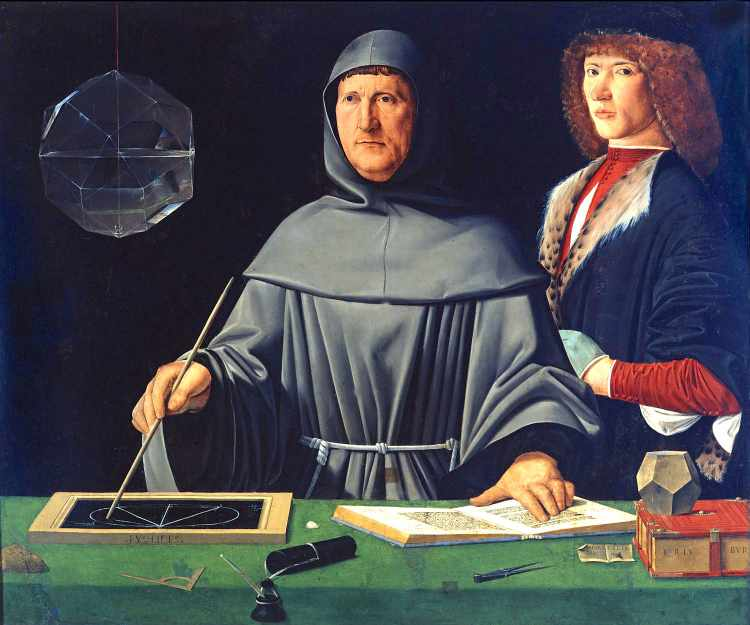
\includegraphics[width=.9\textwidth]{Pacioli.jpg}
\end{minipage}
\begin{minipage}[t]{0.55\textwidth}
  \vspace{0cm}
  Im 15. Jahrhundert wurde in Italien die doppelte Buchführung entwickelt. Dabei wurden Schulden als negative Zahlen notiert. Der italienische Mathematiker und Franziskaner Luca Pacioli hat diese Praxis in seinem Werk \textit{Summa de Arithmetica, Geometria, Proportioni et Proportionalità} festgehalten.
\end{minipage}

% ----------------------------------------------------------------------------
\subsection{Abgeschlossenheit}

Die ganzen Zahlen sind bezüglich der folgenden Operationen abgeschlossen:
\begin{itemize}[noitemsep]
  \item Addition
  \item Subtraktion
  \item Multiplikation
\end{itemize}
Das bedeutet, dass die Summe, die Differenz und das Produkt zweier ganzen Zahlen immer eine ganze Zahl ist.

% ----------------------------------------------------------------------------
\subsection{Teilmengen}
Oft wird über bestimmte Teilmengen der ganzen Zahlen gesprochen. Dabei werden die folgenden Begriffe und Symbole verwendet:
\begin{center}
  \renewcommand{\arraystretch}{1.3}
  \begin{tabularx}{0.8\textwidth}{Xcl}
      \textbf{Begriff}           & \textbf{Symbol}  & \textbf{Menge} \\
    \toprule
      positive ganze Zahlen      & $\mathbb{Z}^{+}$   & $\{1, 2, 3, 4, \ldots\}$ \\
    \midrule
      nichtnegative ganze Zahlen & $\mathbb{Z}_{0}^{+}$ & $\{0, 1, 2, 3, 4, \ldots\} = \mathbb{N}$ \\
    \midrule
      negative ganze Zahlen      & $\mathbb{Z}^{-}$   & $\{\ldots, -4, -3, -2, -1 \}$ \\
    \midrule
      nichtpositive ganze Zahlen & $\mathbb{Z}_{0}^{-}$ & $\{\ldots, -4, -3, -2, -1, 0 \}$ \\
    \bottomrule
  \end{tabularx}
\end{center}

% ----------------------------------------------------------------------------
\subsection{Negative und Gegenzahlen}

Es ist wichtig, negative Zahlen und Gegenzahlen zu unterscheiden. Negative Zahlen sind immer Gegenzahlen von positiven Zahlen. Eine positive Zahl kann aber auch eine Gegenzahl sein. So ist beispielsweise $5$ die Gegenzahl von $-5$.

Wenn eine Variable $a$ verwendet wird, um über eine unbekannte Zahl zu sprechen, so kann es sein, dass die Gegenzahl $-a$ eine positive Zahl ist, nämlich wenn $a$ eine negative Zahl ist.

% ----------------------------------------------------------------------------
\subsection{Rechenregeln}

Für das Rechnen mit Gegenzahlen gelten die folgenden Rechenregeln:
\begin{theorem}
  \textbf{Gegen-Gegenzahl.} Die Gegenzahl der Gegenzahl einer Zahl ist die ursprüngliche Zahl:
  \[
    -(-a) = a
  \]
\end{theorem}
\begin{theorem}
  \textbf{Addition und Subtraktion.} Das Addieren der Gegenzahl ist das Gleiche wie das Subtrahieren der Zahl. Das Subtrahieren der Gegenzahl ist das gleiche wie das Addieren der Zahl.
  \[
    a+(-b) = a-b \qquad\qquad a-(-b) = a+b
  \]
\end{theorem}
\begin{theorem}
  \textbf{Subtraktion einer Summe.} Die Subtraktion einer Summe ist das Gleiche wie das Subtrahieren beider Summanden:
  \[
    a-(b+c) = a-b-c
  \]
\end{theorem}
\begin{theorem}
  \textbf{Subtraktion einer Differenz.} Die Subtraktion einer Differenz ist das Gleiche wie das Subtrahieren des Minuenden und das addieren des Subtrahenden.
  \[
    a-(b-c) = a-b+c
  \]
\end{theorem}
\begin{theorem}
  \textbf{Multiplikation von Gegenzahlen.} Für die Multiplikation von Gegenzahlen gelten folgende Regeln:
  \[
    (-a)\cdot b = a\cdot(-b) = -ab \qquad\qquad  (-a)\cdot(-b) = ab
  \]
\end{theorem}

  \newpage
\section{Division $a:b$}

% ----------------------------------------------------------------------------
\subsection{Definition}

Welche Zahl muss mit Drei multipliziert werden, um Sechs zu erhalten?
\[
  3\cdot\square = 6
\]
Um diese Frage zu beantworten, muss das Verhältnis oder der \textbf{Quotient} von Sechs und Zwei bestimmt werden. Diese wird mit Hilfe einer \textbf{Division} berechnet:
\[
  6 : 3 = \square
\]
\textbf{Definition:} Die Division ist die Umkehroperation der Multiplikation. Mit der Division wird der unbekannte Faktor $x$ einer Multiplikation berechnet:
\begin{align*}
  a\cdot x &= c \\
         x &= c:a
\end{align*}

% ----------------------------------------------------------------------------
\subsection{Schreib- und Sprechweise}

Die Zahl $a$, welche dividiert wird, heisst \textbf{Dividend}. Die Zahl $b$, durch welche dividiert wird, heisst \textbf{Divisor}. Das Resultat einer Division wird \textbf{Quotient} genannt.

Für die Division wird das Operationszeichen $:$ verwendet. Wir schreiben
\[
  a : b = c
\]
und sagen «der Quotient $a$ und $b$ ist gleich $c$.»

% ----------------------------------------------------------------------------
\subsection{Division durch Null}

Die Division durch Null muss speziell betrachtet werden.
\[
  x = c:0
\]
Um das Resultat dieser Division zu bestimmen, wird zunächst die Definition der Division herbeigezogen. Danach ist $x$ die Zahl, welche mit $0$ multipliziert $c$ ergibt:
\[
  x = c:0 \qquad\Leftrightarrow\qquad 0\cdot x = c
\]
Gemäss Definition der Multiplikation ist $0\cdot x$ gleich Null. Wenn also $c$ nicht gleich Null ist, kann keine Zahl für $x$ gefunden werden. Falls jedoch $c$ gleich Null ist, ergibt sich die Frage, was Null geteilt durch Null ergibt. Hier wird wieder die Definition betrachtet:
\[
  x = 0:0 \qquad\Leftrightarrow\qquad 0\cdot x = 0
\]
Das Resultat $x$ der Division von Null durch Null ist also die Zahl, welche mit Null multipliziert Null ergibt. Hier kann jedoch für $x$ jede beliebige Zahl eingesetzt werden.

In beiden Fällen kann keine eindeutige Zahl für $x$ gefunden werden, also ist das Ergebnis einer Division durch Null \textbf{nicht definiert}.

  \input{Brüche}
  \newpage
\section{Rationale Zahlen $\mathbb{Q}$}

Die ganzen Zahlen sind abgeschlossen unter Addition, Multiplikation und Subtraktion. Neh- men wir jetzt allerdings die Division als weitere mögliche Rechenoperation hinzu, so stellen wir fest, dass z.B. das Ergebnis von $5:2$ keine ganze Zahl mehr ist. Auch hier macht die Anwendung oft Probleme: Wie teilt man fünf Äpfel fair auf zwei Personen auf? Was in der Realität auf Probleme stossen mag, lösen die Mathematiker durch Definitionen.

% ----------------------------------------------------------------------------
\subsection{Definition}

Mit welcher Zahl muss Fünf multipliziert werden, um Zwei zu erhalten?
\[
  5\cdot\square = 2
\]
Diese Frage wird mit Hilfe der Umkehroperation, der Division beantwortet. Als Resultat ergibt sich
\[
  \frac{2}{5} = \square
\]
Dieser Bruch ist aber keine ganze Zahl. Somit kann die Frage innerhalb der ganzen Zahlen nicht beantwortet werden.

Das Problem wird gelöst, indem wiederum neue Zahlen «erfunden» werden.

\textbf{Definition:} Ein Bruch mit ganzen Zahlen in Zähler und Nenner heisst \textbf{rationale Zahl}. Dabei darf der Nenner nicht gleich Null sein. In mathematischer Schreibweise ist $r$ eine rationale Zahl, wenn
  \[
    r := \frac{z}{n} \qquad z,n \in \mathbb{Z},\quad n \ne 0
  \]

Werden alle rationalen Zahlen zusammengefasst, ergibt sich die Menge der rationalen Zahlen.

\textbf{Definition:} Die Menge der rationalen Zahlen ist
  \[
    \mathbb{Q} := \left\{ \frac{z}{n} \quad \middle| \quad z,n \in \mathbb{Z}, \quad n \ne 0 \right\}
  \]
\begin{example}
  \textbf{Beispiele:} Einige rationale Zahlen sind
  \[
    \frac{1}{2} \qquad \frac{-4}{-9} \qquad \frac{-5}{10000} \qquad \frac{0}{-2000} \qquad \frac{10}{1}
  \]
\end{example}
\begin{note}
  \textbf{Achtung:} Sogenannte «gemischte Brüche» werden hier nicht definiert. Grundsätzlich sollte die Schreibweise als «gemischter Bruch» vermieden werden, da Sie zu Unklarheiten führen kann. In der Mathematik wird nämlich das Multiplikationszeichen normalerweise weggelassen, nur zwischen zwei Zahlen ist es notwendig. So ist $2a = 2\cdot a$ oder $5\pi = 5\cdot\pi$. Wird nun $2\frac{1}{2}$ geschrieben, so ist unklar, ob dies nun $2+\frac{1}{2}$ oder $2\cdot\frac{1}{2}$ bedeuten soll.

  \textbf{Regel:} Das Additionszeichen darf nicht weggelassen werden, nur das Multiplikationszeichen. «Gemischte Brüche» sind also verboten!
\end{note}

% ----------------------------------------------------------------------------
\subsection{Zahlengerade und Mittelwert}

Auch die rationalen Zahlen lassen sich auf dem Zahlenstrahl darstellen. So befindet sich beispielsweise die Zahl $\frac{1}{2}$ in der Mitte der Zahlen Null und Eins.

\begin{center}
  \begin{tikzpicture}
    \tkzInit[xmin=-2,xmax=2.5,xstep=0.4]
    \tkzDrawX[noticks,label={}]
    \tkzDefPoint(0,0){O}
    \tkzDrawLine({0,-0.1},{0,0.1})
    \tkzLabelPoint({0,-0.1}){$0$}

    \tkzDrawLine({4,-0.1},{4,0.1})
    \tkzLabelPoint({4,-0.1}){$1$}

    \tkzDrawLine({-4,-0.1},{-4,0.1})
    \tkzLabelPoint({-4,-0.1}){$-1$}

    \tkzDrawLine({2,-0.1},{2,0.1})
    \tkzLabelPoint({2,-0.1}){$\frac{1}{2}$}

    \tkzDrawLine({-1.6,-0.1},{-1.6,0.1})
    \tkzLabelPoint({-1.6,-0.1}){$-\frac{2}{5}$}

    \tkzDrawLine({5.33,-0.1},{5.33,0.1})
    \tkzLabelPoint({5.33,-0.1}){$\frac{4}{3}$}
  \end{tikzpicture}
\end{center}
In der Mitte von zwei rationalen Zahlen befindet sich immer deren Mittelwert, der ebenfalls eine rationale Zahl ist. Somit liegen zwischen zwei beliebigen rationalen Zahlen auf dem Zahlenstrahl \textbf{unendlich viele weitere} rationale Zahlen. In der Mathematik wird gesagt, die rationalen Zahlen \textbf{liegen dicht} auf dem Zahlenstrahl.

% ----------------------------------------------------------------------------
\subsection{Abgeschlossenheit}

Die rationalen Zahlen sind bezüglich der folgenden Operationen abgeschlossen:
\begin{itemize}[noitemsep]
  \item Addition
  \item Subtraktion
  \item Multiplikation
  \item Division
\end{itemize}
Das bedeutet, dass die Summe, die Differenz, das Produkt oder der Quotient zweier rationaler Zahlen immer eine rationale Zahl ist.

% ----------------------------------------------------------------------------
\subsection{Äquivalenz}

Brüche können erweitert und gekürzt werden, ohne dass sich deren Wert ändert. Das bedeutet, dass es für jede rationale Zahl unendlich viele verschiedene Darstellungen als Bruch .So ist
\[
  \frac{1}{2} = \frac{2}{4} = \frac{-3}{-6} = \frac{40000}{80000} \cdots
\]
Damit die Darstellung von rationalen Zahlen eindeutig ist, werden folgende Regeln festgelegt:
\begin{itemize}[noitemsep]
  \item Jede rationale Zahl wird durch den \textbf{vollständig gekürzten Bruch} dargestellt.
  \item Ist die rationale Zahl negativ, so wird das \textbf{Minuszeichen vor den Bruch} geschrieben.
  \item Ist der Nenner gleich Eins, wird dieser weggelassen.
\end{itemize}
\begin{example}
  \textbf{Beispiele:}
  \[
    \frac{-4}{-9} = \frac{4}{9}, \qquad \frac{-5}{10} = -\frac{1}{2} \qquad \frac{20}{2} = 10
  \]
\end{example}

% ----------------------------------------------------------------------------
\subsection{Dezimalbrüche}

Jede rationale Zahl kann auch als Dezimalzahl dargestellt werden. Dazu wird das Stellenwertsystem nach rechts erweitert. Rechts von der Stelle Null steht ein Dezimalpunkt, dann folgt die Stelle $-1$, welche einen Stellenwert von $10^{-1}$ oder $\frac{1}{10}$ hat. Wenn wir eine Stelle nach rechts gehen, wird der Stellenwert immer durch Zehn dividiert.

Die Dezimalzahl $42.875$ bedeutet also, dass $4$ Zehner, $2$ Einer, $8$ Zehntel, $7$ Hundertstel und $5$ Tausendstel addiert werden:
\begin{center}
  \renewcommand{\arraystretch}{1.3}
  \newcolumntype{C}{>{\centering\arraybackslash}X}
  \begin{tabularx}{0.9\textwidth}{lCCCCC}
  \toprule
    Stelle & $1$ & $0$ & $-1$ & $-2$ & $-3$ \\
  \midrule
    Stellenwert (Potenz) & $10^{1}$ & $10^{0}$ & $10^{-1}$ & $10^{-2}$ & $10^{-3}$ \\
  \midrule
    Stellenwert & $10$ & $1$ & $\frac{1}{10}$ & $\frac{1}{100}$ & $\frac{1}{1000}$ \\
  \midrule
    Ziffer & $4$ & $2.$ & $8$ & $7$ & $5$ \\
  \midrule
    Wert & $4\cdot 10$ & $2\cdot 1$ & $8\cdot\frac{1}{10}$ & $7\cdot\frac{1}{100}$ & $5\cdot\frac{1}{1000}$ \\
  \bottomrule
  \end{tabularx}
\end{center}
Um einen beliebigen Bruch in eine Dezimalzahl umzuwandeln, wird die schriftliche Division angewendet.
\begin{example}
  \textbf{Beispiele:} Die rationale Zahlen $\frac{1}{8}$, $\frac{2}{3}$ und $\frac{1}{6}$ werden wie folgt als Dezimalbruch dargestellt:
  \[
    \longdivision{1}{8} \qquad\qquad\qquad \longdivision{2}{3} \qquad\qquad\qquad \longdivision{1}{6}
  \]
\end{example}
Manche rationalen Zahlen lassen sich nicht als endliche Dezimalbrüche darstellen, da bei der schriftlichen Division immer ein Rest übrig bleibt. Das heisst, dass sich einige Dezimalstellen unendlich oft wiederholen. Diese werden mit einem Strich oberhalb der Ziffern markiert. Solche Dezimalbrüch heissen \textbf{periodische Dezimalbrüche}.
\begin{example}
  \textbf{Beispiel:} Einige periodische Dezimalbrüche sind:
  \[
    \frac{1}{3} = 0.\overline{3} \qquad
    \frac{1}{6} = 0.1\overline{6} \qquad
    \frac{1}{7} = 0.\overline{142857} \qquad
    \frac{1}{9} = 0.\overline{1} \qquad
    \frac{1}{11} = 0.\overline{09} \qquad
    \frac{1}{13} = 0.\overline{076923}
  \]
\end{example}
Um eine Dezimalzahl in einen Bruch zu verwandeln, rechnen addieren wir einfach die Werte der Dezimalstellen, indem wir die Brüche gleichnamig machen:
\[
  0.875 = \frac{8}{10} + \frac{7}{100} + \frac{5}{1000} = \frac{875}{1000} =\frac{175\cdot 5}{200\cdot 5} = \frac{35\cdot 5}{40\cdot 5} = \frac{7\cdot 5}{8\cdot 5} = \frac{7}{8}
\]

  \newpage
\section{Potenzen mit ganzen Zahlen $(-a)^{-b}$}

% ----------------------------------------------------------------------------
\subsection{Negativer Exponent}

Bisher konnten Potenzen nur eine natürliche Zahl als Exponenten haben. Man kann sich aber fragen, was es bedeuten würde, wenn eine negative Zahl im Exponenten steht. Dazu wird betrachtet, was passiert, wenn bei einer Potenz immer wieder der Exponent um Eins verringert wird.
\begin{align*}
  5^{3} &= 1\cdot 5\cdot 5\cdot 5 = 125 && |\; :5\\
  5^{2} &= 1\cdot 5\cdot 5 = 25         && |\; :5\\
  5^{1} &= 1\cdot 5 = 5                 && |\; :5\\
  5^{0} &= 1
\end{align*}
Wenn bei einer Potenz der Exponent um eins verringert wird, bedeutet dies, dass der Wert der Potenz durch ihre Basis dividiert wird. Das macht Sinn, ein um Eins kleinerer Exponent bedeutet ja, dass die Basis einmal weniger mit sich selbst multipliziert wird.

Wenn nun diese Regel bei der Potenz $5^{0}$ weiter angewendet wird, dann entsteht die Potenz $5^{-1}$. Deren Wert ist der Wert von $5^{0}$ dividert durch $5$ also $\frac{1}{5}$. Wird dies so fortgesetzt, können die Werte für sämtliche Potenzen mit negativem Exponenten bestimmt werden:
\begin{align*}
  5^{0}    &= 1                               && |\; :5\\\\
  5^{-1} &= \frac{1}{5}                       && |\; :5\\\\
  5^{-2} &= \frac{1}{5\cdot 5} = \frac{1}{25} && |\; :5\\\\
  5^{-3} &= \frac{1}{5\cdot 5\cdot 5} = \frac{1}{125}
\end{align*}

Diese Überlegungen werden in folgender Definition festgehalten:

\textbf{Definition:} Die Potenz einer Zahl $a$ mit einem negativen Exponenten $-n$ ist der Kehrwert der Potenz mit der Gegenzahl $n$ im Exponenten.
\[
  a^{-n} := \frac{1}{a^{n}} = \frac{1}{1\cdot\underbrace{a\cdot a\cdot a\cdots a}_{n-\text{mal}}}
\]

\begin{example}
  \textbf{Beispiele:} $\displaystyle \qquad 4^{-7} = \frac{1}{4^{7}} \qquad\qquad 3^{-1} = \frac{1}{3} \qquad\qquad 10^{-2} = \frac{1}{10^{2}} = 0.01$
\end{example}

\newpage
% ----------------------------------------------------------------------------
\subsection{Negative Basis}

Im folgenden wird betrachtet, welche Werte die Potenz einer negativen Zahl annimmt, indem die Definition angewendet wird.
\begin{align*}
  (-5)^{0} &= 1 = -5^{0} \\
  (-5)^{1} &= 1\cdot(-5) = -5^{1} \\
  (-5)^{2} &= 1\cdot(-5)\cdot(-5) = 25 = 5^{2} \\
  (-5)^{3} &= 1\cdot(-5)\cdot(-5)\cdot(-5) = -125 = -5^{3} \\
  (-5)^{4} &= 1\cdot(-5)\cdot(-5)\cdot(-5)\cdot(-5) = 625 = 5^{4}
\end{align*}
Wenn zwei negative Zahlen multipliziert werden, ergibt sich eine positive Zahl. Wenn der Exponent gerade ist, können alle Faktoren paarweise multipliziert werden und das Resultat ist positiv. Wenn der Exponent ungerade ist, bleibt immer ein negativer Faktor übrig.

\begin{theorem}
  Die Potenz einer negativen Zahl $-n$ mit einem \textbf{geraden Exponenten} $b$ ist gleich der Potenz mit der Gegenzahl $n$ als Basis.
  \[
    (-n)^{b} = n^{b} \qquad \text{wenn}\;b\;\text{gerade}
  \]
  Die Potenz einer negativen Zahl $-n$ mit einem \textbf{ungeraden Exponenten} $b$ ist gleich der Gegenzahl der Potenz mit der Gegenzahl $n$ als Basis.
  \[
    (-n)^{b} = -n^{b} \qquad \text{wenn}\;b\;\text{ungerade}
  \]
\end{theorem}

% ----------------------------------------------------------------------------
\subsection{Potenzgesetze}

Potenzen können gemäss der fünf Potenzgesetze umgeformt werden.

\begin{theorem}
  \textbf{Produkt mit gleicher Basis.} Potenzen mit gleicher Basis werden multipliziert, indem die Potenzen addiert werden:
  \[
    a^{k} \cdot a^{m} = a^{k+m}
  \]
\end{theorem}

\textbf{Begründung:} Gemäss der Definition der Potenz bedeutet $a^{k}$, dass $a$ der Faktor $k$-mal in der Multiplikation vorkommt. $a^{m}$ bedeutet, dass der Faktor $m$-mal vorkommt. Insgesamt kommt der Faktor $a$ also $(k+m)$-mal in der Multiplikation vor. Dies kann gemäss Definition wiederum als $a^{k+m}$ geschrieben werden.
\[
  a^{k}\cdot a^{m} = 1\cdot\underbrace{a\cdot a\cdot a\cdots a}_{k-\text{mal}}\cdot 1\cdot\underbrace{a\cdot a\cdot a\cdots a}_{m-\text{mal}} = 1\cdot\underbrace{a\cdot a\cdot a\cdots a}_{(k+m)-\text{mal}} = a^{k+m}
\]

\begin{example}
  \textbf{Beispiele:}
  \[
    5^{2}\cdot 5^{3} = 5^{2+3} = 5^{5} \qquad\qquad 3\cdot 3^{-3} = 3^{1+(-3)} = 3^{-2}
  \]
\end{example}
\vspace{1cm}

\begin{theorem}
  \textbf{Quotient mit gleicher Basis.} Potenzen mit gleicher Basis werden dividiert, indem die Potenzen subtrahiert werden:
  \[
    \frac{a^{k}}{a^{m}} = a^{k-m}
  \]
\end{theorem}

\textbf{Begründung:} Gemäss der Definition der Potenz bedeutet $a^{k}$, dass $a$ der Faktor $k$-mal vorkommt. $a^{m}$ bedeutet, dass der Faktor $m$-mal vorkommt. Insgesamt kommt der Faktor $a$ also $k$-mal im Zähler und $m$-mal im Nenner vor. Ist $k$ grösser als $m$, so bleibt der Faktor $(k-m)$-mal im Zähler übrig, was als $a^{k-m}$ geschrieben werden kann.
\[
  \frac{a^{k}}{a^{m}} = \frac{1\cdot\overbrace{a\cdot a\cdot a\cdots a}^{k-\text{mal}}}{1\cdot\underbrace{a\cdot a\cdots a}_{m-\text{mal}}} = \frac{1\cdot\overbrace{a\cdot a\cdots a}^{(k-m)-\text{mal}}}{1} = a^{k-m}
\]
Ist hingegen $m$ grösser als $k$, so bleibt der Faktor $(m-k)$-mal im Nenner übrig. Dies kann im Nenner als $a^{m-k}$ geschrieben werden. Dank der Definition der Potenz für negative Exponenten kann dies ebenfalls zu $a^{k-m}$ umgeformt werden.
\[
  \frac{a^{k}}{a^{m}} = \frac{1\cdot\overbrace{a\cdot a\cdot a\cdots a}^{k-\text{mal}}}{1\cdot\underbrace{a\cdot a\cdots a}_{m-\text{mal}}} = \frac{1}{1\cdot\underbrace{a\cdot a\cdots a}_{(m-k)-\text{mal}}} = \frac{1}{a^{m-k}} = a^{-(m-k)} = a^{k-m}
\]

\begin{example}
  \textbf{Beispiele:} $\displaystyle \frac{5^{2}}{5^{3}} = 5^{2-3} = 5^{-1} \qquad\qquad \frac{3^{-2}}{3^{-4}} = 3^{-2-(-4)} = 3^{2}$
\end{example}

\begin{theorem}
  \textbf{Produkt mit gleichem Exponent.} In einem Produkt können gleiche Exponenten ausgeklammert werden:
  \[
    a^{k}\cdot b^{k} = (a\cdot b)^{k}
  \]
\end{theorem}

\textbf{Begründung:} Gemäss Definition ist $a^{k}\cdot b^{k}$ ein Produkt, in welchem die Faktoren $a$ und $b$ je $k$-mal vorkommen. Wegen der Kommutativität der Multiplikation können die Faktoren umgestellt werden, sodass $k$ Faktoren $(a\cdot b)$ entstehen. Dieses Produkt kann wiederum als $(a\cdot b)^{k}$ geschrieben werden.
\[
  a^{k}\cdot b^{k} = 1\cdot\underbrace{a\cdot a\cdot a\cdots a}_{k-\text{mal}}\cdot 1\cdot\underbrace{b\cdot b\cdot b\cdots b}_{k-\text{mal}} = 1\cdot\underbrace{(a\cdot b)\cdot (a\cdot b)\cdot (a\cdot b)\cdots (a\cdot b)}_{k-\text{mal}} = (ab)^{k}
\]

\begin{example}
  \textbf{Beispiele:} $\displaystyle 5^{3} \cdot 3^{3} = (5\cdot 3)^{3} = 15^{3} \qquad\qquad 2^{-2}\cdot 7^{-2} = (2\cdot 7)^{-2} = 14^{-2}$
\end{example}

\begin{theorem}
  \textbf{Quotient mit gleichem Exponent.} In einem Bruch können gleiche Exponenten ausgeklammert werden:
  \[
    \frac{a^{k}}{b^{k}} = \left(\frac{a}{b}\right)^{k}
  \]
\end{theorem}

\textbf{Begründung:} Gemäss Definition hat der Bruch $\frac{a^{k}}{b^{k}}$ im Zähler bzw. im Nenner $k$ Faktoren $a$ bzw. $b$. Der Bruch kann also in eine Multiplikation von $k$ Brüchen $\frac{a}{b}$ aufgeteilt werden. Diese können gemäss Definition der Potenz als $\left(\frac{a}{b}\right)^{k}$ geschrieben werden.
\[
  \frac{a^{k}}{b^{k}} = \frac{1\cdot\overbrace{a\cdot a\cdot a\cdots a}^{k-\text{mal}}}{1\cdot\underbrace{b\cdot b\cdot b\cdots b}_{k-\text{mal}}} = 1\cdot\underbrace{\frac{a}{b}\cdot \frac{a}{b}\cdot \frac{a}{b}\cdots \frac{a}{b}}_{k-\text{mal}} = \left(\frac{a}{b}\right)^{k}
\]

\begin{example}
  \textbf{Beispiele:} $\displaystyle \frac{4^{6}}{2^{6}} = \left(\frac{4}{2}\right)^{6} = 2^{6} \qquad\qquad \frac{3^{-2}}{5^{-2}} = \left(\frac{3}{5}\right)^{-2} = 0.6^{-2}$
\end{example}

\begin{theorem}
  \textbf{Potenz einer Potenz.} Potenzen werden potenziert, indem die Exponenten multipliziert werden:
  \[
    \left(a^{k}\right)^{m} = \left(a^{m}\right)^{k}= a^{k\cdot m}
  \]
\end{theorem}

\textbf{Begründung:} $a^{k}$ bedeutet, dass der Faktor $a$ im Produkt $k$-mal vorkommt. Wird die Potenz nochmals mit $m$ potenziert, bedeutet dies, dass alle $k$ Faktoren $m$-mal wiederholt werden. Insgesamt kommt der Faktor $a$ in $\left(a^{k}\right)^{m}$ also $(k\cdot m)$-mal vor. Dies kann auch als $a^{k\cdot m}$ geschrieben werden.
\[
  (a^{k})^{m} = \overbrace{1\cdot\underbrace{a\cdot a\cdots a}_{k-\text{mal}}\cdot 1\cdot\underbrace{a\cdot a\cdots a}_{k-\text{mal}}\cdots 1\cdot\underbrace{a\cdot a\cdots a}_{k-\text{mal}}}^{m-\text{mal}} = 1\cdot\underbrace{a\cdot a\cdot a\cdots a}_{(k\cdot m)-\text{mal}} = a^{k\cdot m}
\]

\begin{example}
  \textbf{Beispiele:} $\displaystyle (2^{3})^{2} = 2^{3\cdot 2} = 2^{6} \qquad\qquad (5^{2})^{-2} = 5^{2\cdot(-2)} = 5^{-4}$
\end{example}

\begin{note}
  \textbf{Achtung:} Potenzen werden von oben nach unten berechnet. So ist $5^{3^{2}}$ nicht dasselbe wie $\left(5^{3}\right)^{2}$:
  \[
    5^{3^{2}} = 5^{\left(3^{2}\right)} = 5^{9} \qquad\qquad \left(5^{3}\right)^{2} = 5^{3\cdot 2} = 5^{6}
  \]
\end{note}

  \input{Wissenschaftliche Schreibweise und Präfixe}
  \newpage
\section{Quadratwurzeln $\sqrt{a}$}

% ----------------------------------------------------------------------------
\subsection{Definition}

Welche Zahl muss quadriert werden, um Neun zu erhalten?
\[
  \square^{2} = 9
\]
Diese Frage wird mit Hilfe der Umkehroperation, dem Wurzelziehen oder Radizieren, beantwortet. Als Resultat ergibt sich
\[
  \sqrt{9} = \square
\]
Dabei ist zu beachten, dass es zwei Zahlen gibt, deren Quadrat Neun ist, nämlich $3$ und $-3$. Damit das Wurzelziehen eindeutig ist, wird festgelegt, dass das eine Wurzel nie negativ sein kann.

Welche Zahl muss quadriert werden, um $-9$ zu erhalten?
\[
  \square^{2}= -9
\]
Das ein Quadrat nie negativ sein kann, gibt es keine Antwort auf diese Frage. Das Wurzelziehen aus negativen Zahlen ist somit nicht definiert.


\textbf{Definition:} Das Wurzelziehen oder Radizieren ist die Umkehroperation des Quadrierens. Mit dem Radizieren wird die unbekannte, nicht-negative Basis eines Quadrates berechnet:
\begin{align*}
  x^{2} &= a \qquad\qquad x\ge 0\\
      x &= \sqrt{a} \qquad\qquad a\ge 0
\end{align*}
Das Radizieren einer negativen Zahl ist nicht definiert.

\begin{example}
  \textbf{Beispiele:} $\sqrt{25} = 5 \qquad \sqrt{0} = 0 \qquad \sqrt{1} = 1 \qquad \sqrt{-4}$ ist nicht definiert.
\end{example}


% ----------------------------------------------------------------------------
\subsection{Schreib- und Sprechweise}

Die Zahl $a$ welche radiziert wird, heisst \textbf{Radikand}. Das Resultat des Wurzelziehens heisst \textbf{Wurzel} oder \textbf{Radikal}.

Für das Wurzelziehen wird das Operationszeichen $\sqrt{\phantom{x}}$ verwendet. Wir schreiben
\[
  \sqrt{a} = b
\]
und sagen «Die Wurzel von $a$ ist gleich $b$.»

\begin{example}
  \textbf{Beispiel:} Die Wurzel von $49$ ist Sieben: $\sqrt{49} = 7$
\end{example}

% ----------------------------------------------------------------------------
\subsection{Gesetze}

Wurzeln können gemäss der folgenden Gesetze umgeformt werden.

\begin{theorem}
  \textbf{Produktregel.} Das Produkt zweier Wurzeln ist gleich der Wurzel aus dem Produkt der beiden Radikanden.
  \[
    \sqrt{a}\cdot\sqrt{b} = \sqrt{a\cdot b}
  \]
  Das Produkt zweier gleicher Wurzeln ist gleich dem Radikanden:
  \[
    \sqrt{a}\cdot\sqrt{a} = a
  \]
\end{theorem}

\begin{example}
  \textbf{Beispiele:} $\displaystyle \sqrt{3}\cdot\sqrt{5} = \sqrt{3\cdot 5} = \sqrt{15} \qquad\qquad \sqrt{2}\cdot\sqrt{2} = \sqrt{2\cdot 2} = \sqrt{4} = 2$
\end{example}

\begin{theorem}
  \textbf{Quotientenregel.} Der Quotient zweier Wurzeln ist gleich der Wurzel des Quotienten der beiden Radikanden.
  \[
    \frac{\sqrt{a}}{\sqrt{b}} = \sqrt{\frac{a}{b}}
  \]
\end{theorem}

\begin{example}
  \textbf{Beispiele:} $\displaystyle \frac{\sqrt{2}}{\sqrt{5}} = \sqrt{\frac{2}{5}} \qquad\qquad \frac{\sqrt{27}}{\sqrt{3}} = \sqrt{\frac{27}{3}} = \sqrt{9} = 3$
\end{example}

\begin{theorem}
  \textbf{Quadrieren einer Wurzel.} Das Quadrat einer Wurzel ist gleich dem Radikanden. Dabei muss natürlich beachtet werden, dass der Radikand nicht negativ sein kann.
  \[
    \left(\sqrt{a}\right)^{2} = a \qquad a\ge 0
  \]
\end{theorem}

\begin{example}
  \textbf{Beispiele:} $\displaystyle \left(\sqrt{5}\right)^{2} = 5 \qquad\qquad \sqrt{3}\cdot\sqrt{3} = \left(\sqrt{3}\right)^{2} = 3$
\end{example}

\begin{theorem}
  \textbf{Wurzel eines Quadrats.} Die Wurzel eines Quadrats ist gleich dem Betrag der Basis.
  \[
    \sqrt{a^{2}} = |a|
  \]
\end{theorem}
Hier kann $a$ durchaus eine negative Zahl sein, da ja der Radikand $a^{2}$ in jedem Fall positiv ist. Da das Resultat der Wurzel gemäss Definition nicht negativ sein kann, muss hier der Betrag von $a$ genommen werden.

\begin{example}
  \textbf{Beispiele:} $\displaystyle \sqrt{5^{2}} = |5| = 5 \qquad\qquad \sqrt{(-3)^{2}} = |-3| = 3$
\end{example}

  \newpage
\section{Reelle Zahlen $\mathbb{R}$}

So wie uns die Subtraktion von den natürlichen Zahlen zu den ganzen Zahlen geführt hat und wir mit der Division auf die rationalen Zahlen gestossen sind, so führt das Wurzelziehen zu den reellen Zahlen. Denn leider ist die Wurzel aus einer rationalen Zahl nicht immer eine rationale Zahl. Das berühmteste Beispiel hierfür ist sicher $\sqrt{2}$.

% ----------------------------------------------------------------------------
\subsection{irrationale Zahlen}

Wir haben gesehen, dass die rationalen Zahlen auf der Zahlengerade dicht liegen. Das heisst, wir finden zwischen zwei rationalen Zahlen immer unendlich viele weitere.

Wir können aber auch Zahlen konstruieren, die nicht rational sind. Dazu müssen wir nur eine unendliche Dezimalentwicklung angeben, die nicht periodisch ist, beispielsweise:
\[
  0.1011011101111011111011111101\ldots
\]

Diese Zahl liegt natürlich auch auf der Zahlengerade, zwischen $0.1$ und $0.11$, sie ist aber nicht eine rationale Zahl, da sie nicht als Bruch darstellbar ist.

\textbf{Definition:} Eine Zahl auf der Zahlengeraden, welche nicht eine rationale Zahl ist, also \textbf{nicht} in der Form
\[
  \frac{z}{n} \qquad z \in \mathbb{Z},\quad n \in \mathbb{Z^{+}}
\]
geschrieben werden kann, heisst \textbf{irrationale} Zahl.

Werden alle rationalen und alle irrationalen Zahlen zusammengefasst, ergeben sich sämtliche Zahlen auf der Zahlengeraden.

\textbf{Definition:} Alle rationalen und irrationalen Zahlen zusammen werden \textbf{reelle Zahlen} genannt und mit $\mathbb{R}$ bezeichnet.

% ----------------------------------------------------------------------------
\subsection{Beweis der Irratonalität von Zahlen}

Es ist gar nicht so einfach zu beweisen, dass eine bestimmte Zahl irrational ist.

\begin{itemize}
  \item Dass $\sqrt{2}$ und weitere Wurzeln irrational sind, hat der Grieche Archytas von Tarent ca. 420 v. Chr. bewiesen.
  \item Dass die Kreiszahl $\pi$ irrational ist, hat Johann Heinrich Lambert 1761 bewiesen.
  \item Dass die eulersche Zahl $e$ irrational ist, hat Charles Hermite 1873 bewiesen.
  \item Bei anderen Zahlen wird die Irrationalität vermutet, ist aber bis heute nicht bewiesen, z.B. bei
  \[
    \pi + e \qquad\qquad \pi - e \qquad\qquad \pi^{\pi}
  \]
\end{itemize}

\newpage
% ----------------------------------------------------------------------------
\subsection{Irrationalität von Wurzeln}

Der Beweis, dass bestimmte Wurzeln irrational sind, ist von Euklid überliefert worden und ist relativ einfach nachvollziehbar, hier am Beispiel von $\sqrt{5}$

\begin{theorem}
  \textbf{Satz:} Die Wurzel von fünf ist keine rationale Zahl.
\end{theorem}

\textbf{Beweis:} Der Satz wird mit einem Widerspruchsbeweis bewiesen. Das bedeutet, dass das Gegenteil angenommen und gezeigt wird, dass diese Annahme zu einem Widerspruch führt.

Es wird also angenommen, dass $\sqrt{5}$ eine rationale Zahl ist. Jede rationale Zahl kann als vollständig gekürzten Bruch dargestellt werden:
\[
  \sqrt{5} = \frac{z}{n} \qquad z \in \mathbb{Z}, \quad n \in \mathbb{Z^{+}}
\]

Nun wird die Gleichung auf beiden Seiten quadriert:
\[
  5 = \left(\frac{z}{n}\right)^{2} = \frac{z^{2}}{n^{2}}
\]
Die Gleichung kann wie folgt geschrieben werden:
\[
  \frac{5}{1} = \frac{z^{2}}{n^{2}}
\]
Diese Gleichung hat auf beiden Seiten einen vollständig gekürzten Bruch, da $z$ und $n$ gemäss Annahme keine gemeinsamen Teiler haben. Zwei vollständig gekürzte Brüche sind gleich, wenn Zähler und Nenner gleich sind. Also folgt:
\[
  5 = z^{2} \qquad\text{und}\qquad 1 = n^{2}
\]
Es gibt aber keine ganze Zahl $z$, deren Quadrat $5$ ist. Damit ist ein Widerspruch aufgezeigt worden. Daraus folgt, dass die Annahme, dass $\sqrt{5}$ eine rationale Zahl ist, falsch sein muss.
\begin{note}
  \textbf{Anmerkung:} Um den Beweis richtig nachvollziehen zu können ist wichtig zu verstehen, was es bedeutet, dass der Bruch $\frac{n}{z}$ vollständig gekürzt ist. Dies bedeutet, dass $z$ und $n$ keine gemeinsamen Teiler haben, die noch gekürzt werden könnten. Insbesondere sind in der Primfaktorzerlegung alle Primfaktoren von $z$ und $n$ verschieden. Beim Quadrieren einer Zahl kommen keine neuen Primfaktoren hinzu, die vorhandenen Primfaktoren werden nur jeweils verdoppelt. Deshalb haben auch $z^{2}$ und $n^{2}$ keinen gemeinsamen Teiler und der Bruch $\frac{z^{2}}{n^{2}}$ ist ebenfalls ein gekürzter Bruch.
\end{note}

% ----------------------------------------------------------------------------
\subsection{Intervalle}

Manchmal soll ein Intervall auf der Zahlengeraden beschrieben werden, beispielsweise alle Zahlen zwischen $-1$ und $1$. Dabei muss angegeben werden, ob die Grenzen des Intervalls dazu gerechnet werden oder nicht.

Es werden die folgenden Begriffe und Schreibweisen verwendet:

\begin{center}
  \renewcommand{\arraystretch}{1.1}
  \begin{tabularx}{0.9\textwidth}{XXX}
    \textbf{Begriff} & \textbf{Schreibweise} & \textbf{Definition} \\
  \toprule
    geschlossenes Intervall & $[a, b]$ & $\{ x\in\mathbb{R} \;|\; a \leq x \leq b\}$ \\
  \midrule
    linksoffenes Intervall & $(a, b]$ oder $]a, b]$ & $\{ x\in\mathbb{R} \;|\; a< x \leq b\}$ \\
  \midrule
    rechtsoffenes Intervall & $[a, b)$ oder $[a, b[$ & $\{ x\in\mathbb{R} \;|\; a \leq x < b\}$ \\
  \midrule
    offenes Intervall & $(a, b)$ oder $]a, b[$ & $\{ x\in\mathbb{R} \;|\; a< x < b\}$ \\
  \bottomrule
  \end{tabularx}
\end{center}

Linksoffene und rechtsoffene Intervalle werden zusammen auch als halboffene Intervalle bezeichnet.

% ----------------------------------------------------------------------------
\subsection{Näherungen}

Irrationale Zahlen können wir nicht exakt als Dezimalzahl notieren. In diesem Fall geben wir eine Annäherung an und verwenden wir das Zeichen $\approx$ um zu verdeutlichen, dass die Angabe nicht exakt ist:
\[
  \sqrt{2} \approx 1.414 \qquad\qquad \pi \approx 3.141
\]

%  \input{Abzählbarkeit}
\end{document}
